% gvim: encoding=utf8

\documentclass[11pt, french, screen, research-development]{report-rd-info}
   % - 11pt:  12pt peut être préférable pour faciliter la lecture sur les petits écrans, demander à l'encadrement
   % - french:  à remplacer par english en cas de rédaction (exceptionnelle) en anglais
   % - screen:  à enlever pour obtenir un rapport au format A4
   % - research-development:  à remplacer par 'research' seul, ou 'development' seul, voire 'intelligence' en fonction de la demande du jury à l'issue du travail
\usepackage[utf8]{inputenc}
   % - utf8, latin1, latin9, etc.
\usepackage[T1]{fontenc}

% définitions propres au  contenu actuel
\usepackage{amsmath, amssymb}
\usepackage{algorithm}
   \floatname{algorithm}{Algorithme}
   \ifenglish\renewcommand{\listalgorithmname}{List of Algorithms}
   \else     \renewcommand{\listalgorithmname}{Liste des algorithmes}
   \fi
\usepackage{listings}
   \lstset{backgroundcolor={\color{yellow}},
           columns=fullflexible,
           commentstyle={\color{blue}},
           numbers=left,
           numbersep=5pt,
           numberstyle={\tiny},
           stepnumber=1}
\usepackage{algorithmic}
\usepackage{xcolor}
\usepackage{float}
\usepackage{url}
\usepackage{amsthm}
\usepackage{amssymb}
\usepackage{graphicx}

\newenvironment{typographie}{\begin{quote}\textbf{Typographie}. }{\end{quote}}
\newenvironment{structuration}{\begin{quote}\textbf{Structuration}. }{\end{quote}}
\newenvironment{important}{\begin{quote}\textbf{Important}. }{\end{quote}}

\newenvironment{explanation}
{\color{blue}
 \begin{list}{}{\hspace{0.2\textwidth}\color{blue}}\item $\bullet\bullet\bullet$
}
{\end{list}}


\newenvironment{textClassique}
{\color{black}
 \begin{list}{}{\hspace{0.2\textwidth}\color{black}}\item
}
{\end{list}}


\newtheorem{theoreme}{Théorème}
\newtheorem{preuve}{Preuve}

\begin{document}

\title{GSITM Apprentissage Contrastif}
\subtitle{Rapport de PRED 2026-2027}
\authorA{Floran}{Martel}
\authorB{Matis}{Hadet}
\supervisor{Claudia}{Marinica}
   % Si plusieurs co-encadrants, alors utiliser la forme suivante~:
   %    \cosupervisor{Alter}{Ego \& {\normalfont Jean} Cadre}
% \coordinator{Jean}{Registre}
\institution{LS2N}
   % - LS2N pour un encadrement par les membres des équipes du département (voire d'autres équipes du LS2N) ;
   % - XXX pour un encadrement dans le cadre d'un autre organisme
   %   (il faut alors fournir dans le répertoire "logos" les fichiers correspondant~: XXX.pdf -- à défaut XXX.jpeg ou XXX.png -- pour pdflatex *et* XXX.eps pour latex) ;
   % - commenter pour un encadrement qui relève d'un travail de recherche non affecté à une équipe.
\theme{\'Equipe DUKE}
   % - à fournir dans le cas d'un laboratoire (DUKE, IPI ou RIO pour les équipes du département)
   % - commenter autrement
   % - ne peut pas être fourni si l'institution n'a pas été renseignée
\coinstitution{Centre national de la recherche scientifique}{CNRS}{1.7cm}
   % - pour ajouter un partenaire
   % - le logo doit correspondre au fichier déclaré, ici CNRS.pdf.
   % - le troisième paramètre permet d'adapter la largeur du logo afin
   %   de le rendre visuellement comparable à ceux mis par défaut
   %   (université de Nantes et éventuellement laboratoire)
\date{15 octobre 2026}
   % - inutile de mettre un 0 devant les jours 1 à 9 du mois~!
   % - en français les mois ne prennent pas de majuscule (sauf si vous ne mettez pas le jour)
   % - le jour est peut-être même une précision inutile...

%--------------------------------------------------------------------------------

\begin{abstract}
\small

\begin{textClassique}
   Comme son nom l'indique, le résumé condense en \emph{quelques lignes}, c'est-à-dire au maximum sur cette colonne, la \emph{totalité} du rapport.
   Il faut donc décrire succinctement et successivement, tout ou partie de ce qui suit~:
   \begin{itemize}
      \item le sujet et la problématique~;
      \item les objectifs fixés~;
      \item les recherches effectuées~;
      \item les décisions prises~;
      \item les constructions conceptuelles~;
      \item les développements accomplis~;
      \item les expérimentations conduites, leurs résultats et leur interprétation~;
      \item les limites de ce travail~;
      \item les perspectives qu'il ouvre~;
   \end{itemize}
   sans s'embarrasser de détails inutiles et en restant très vulgarisateur.
   L'introduction et la conclusion du rapport permettent de s'étendre.
\end{textClassique}
\end{abstract}

\begin{classification}
\small
\begin{explanation}
   Des éléments d'indexation bibliographiques \emph{doivent} être fournis.
   Ci-dessous est illustrée l'usage du thésaurus de l'ACM avec les catégories codifiées et des éléments d'indexation ouverts.
   Suivre le modèle de l'ACM~: cf.~\url{http://www.acm.org/class/1998/}

   \category{H.2.8}{Database Applications}{Image databases}
   \category{H.3.3}{Information Search and Retrieval}{Clustering, Information filtering, Relevance feedback}
   \category{H.3.7}{Digital Libraries}{User issues}
   \category{I.5.3}{Clustering}{Algorithms, Similarity measures}
   \category{I.4.10}{Image Representation}{Statistical, Multidimensional}
   \terms{Des mots clés couramment employés et très généraux sont à ajouter aux catégories. ex.~: Algorithms, performance, experimentation, human factors, verification.}
   \keywords{Des mots clés supplémentaires et très spécifiques peuvent être ajoutés. ex.~: Personnalisation, recherche d'images par le contenu, classification, rétro-action,
   apprentissage.}
\end{explanation}
\end{classification}

\maketitle

%--------------------------------------------------------------------------------

\begin{acknowledgements}
\begin{explanation}
   Si le c\oe ur vous en dit... mais leur absence en dit beaucoup.

   En cas de remerciements à plusieurs personnes, n'hésitez pas à utiliser les commodités de l'ordre alphabétique pour ne froisser personne.
\end{explanation}
\end{acknowledgements}

%--------------------------------------------------------------------------------

\newpage

\tableofcontents

%--------------------------------------------------------------------------------

\chapter*{Préambule}
\addcontentsline{toc}{chapter}{Préambule}

\begin{explanation}
   Ce document est pré-rempli avec des explications sur sa structure.
   Tous les paragraphe bleus, endentées et précédées de trois points sont fournis~:
   \begin{itemize}
      \item soit à titre d'illustration~;
      \item soit à titre d'explication.
   \end{itemize}
   En conséquence, rien ne doit en demeurer, si ce n'est la structure logique.
   Il vous est conseillé de les conserver tant que tous les points qui y sont notés n'ont pas été satisfaits afin d'éviter d'en oublier dans le document final.

   \bigskip

   Un préambule est optionnel.
   Il permet d'éclaircir le lecteur sur l'objet du rapport et du travail, son contexte et d'autres aspects périphériques au contenu lui-même (ex.~: les motivations de ce choix de sujet).

   Ici, il nous permet de préciser~:
   \begin{itemize}
      \item quelques points très généraux sur l'écriture d'un rapport, sujet de ce modèle~;
      \item de préciser, dans la mesure du possible, ce qui est attendu en différentes parties du rapport.
   \end{itemize}

   \bigskip

   Tout d'abord, un document \emph{structuré} présente, comme l'indique l'épithète, une structure issue d'un travail d'organisation \emph{réfléchi}.
   Cette organisation peut être propre à un travail particulier mais, le plus souvent, elle obéit à un modèle bien établi (ex.~: le format <<~thèse-antithèse-synthèse~>> d'une dissertation -- même si ce n'est pas le seul).

   Pour un informaticien, cette structure correspond au concept bien connu d'arbre que l'on retrouve clairement dans la table des matières qui précède.

   Il convient alors de distinguer les feuilles de l'arbre des n\oe uds internes ainsi que de la structure hiérarchique par elle-même.

   Les feuilles portent les informations factuelles ou techniques, les séquences d'une démonstration, etc.
   Bref, elles constituent le c\oe ur du rapport, le contenu à proprement parler.

   L'arbre lui-même décrit l'organisation logique du raisonnement.
   Dans le cas le plus simple, cela va des hypothèses à la conclusion, les imbrications correspondant à des niveaux de détails.
   Dans d'autres cas, la structure hiérarchique traduit tant bien que mal des présentations plus pertinentes mais qui ne s'accommodent pas de la linéarité du texte.
   Par exemple, certaines présentations nécessitent, pour être parfaitement claires, une organisation bidimensionnelle.
   Il faut alors choisir de présenter ce tableau ligne par ligne, colonne par colonne ou encore blocs par blocs.
   Lorsque ce genre de situation se présente, une explication préalable sur la logique <<~naturelle~>> et la logique de linéarisation adoptée est indispensable.
   La fin de l'introduction, où se trouve placé le plan de l'étude, est l'endroit où justifier la logique de linéarisation.

   Ainsi, les n\oe uds internes de cet arbre soulignent-ils seulement les étapes dans le développement des idées.
   Chaque n\oe ud interne doit alors donner lieu à~:
   \begin{itemize}
      \item une introduction au contenu de son sous-arbre~;
      \item une liaison entre les développements de chacune de ses branches~;
      \item une conclusion locale.
   \end{itemize}
   Cette structure, récursive de surcroît, amène à de nombreuses redites, mais à des niveaux de détails différents.
   Elle est indispensable, car ce sont ces annonces, liaisons et récapitulatifs qui permettent au lecteur de savoir (i)~ce qui l'attend dans la suite et (ii)~à quel niveau il se situe à chaque instant.
   L'usage rigoureux et discipliné de cette écriture <<~hiérarchique~>> dans le cadre réducteur d'une écriture réelle <<~linéaire~>> permettrait même de se dispenser de toute marque claire dans le texte.
   (Certains ouvrages scientifiques ont effectivement été rédigés, à l'instar des romans, avec comme unique niveau de découpage le chapitre~!)

   Nous en déduisons donc que les titres de chapitres, sections, etc., ne sont \emph{pas} du texte.
   Il s'agit exclusivement de délimiteurs visuels qui soulignent à leur façon les niveaux hiérarchiques.
   Dans le cours d'une lecture normale, \emph{l'\oe il les saute}.

   Il est donc interdit d'utiliser un pronom qui fait référence au contenu d'un titre.
   Par exemple, après une section intitulée <<~Base de données~>> (on notera l'absence d'article), le paragraphe suivant ne commencera jamais par <<~Elle [...]~>> mais bien par <<~La base de données [...]~>>.

   \begin{typographie}
   Soulignons aussi que des règles typographiques de mise en page et de mise en forme existent.
   Certaines d'entre-elles concernent la numérotation, la taille, la graisse, etc., des titres.
   Il se trouve que le système de publication \LaTeX, utilisé pour ce même document, les respectent, sous une forme conventionnelle et sobre que vous constatez \emph{de visu}.
   En cas d'utilisation d'un autre outil de rédaction de texte électronique, il faut forcer ce dernier à respecter des règles analogues (\emph{via} des feuilles de style de préférence mais pas nécessairement celles fournies par défaut...
   car elles sont généralement aux normes américaines).

   Dans la suite, nous ajouterons encore aux recommandations sur la technique de construction du rapport lui-même des remarques sur les règles typographiques au sens large, même si elles nécessiteraient une présentation dédiée.
   \end{typographie}

   \bigskip

   Dans la suite, certaines parties de ce pseudo rapport ont été rédigées d'une manière très proche de la forme finale.
   En revanche, d'autres parties ne donnent que des indications très grossières, voire seulement des exemples (mis en italique), car leur contenu est très dépendant de la nature du sujet et des résultats.

   \bigskip

   Faisons une dernière recommandation, qui va de soi mais sur laquelle il convient d'insister néanmoins~: il faut rédiger en français.
   Cela englobe la correction orthographique (les erreurs orthographiques sont \emph{totalement} inacceptables), grammaticale et... l'absence de franglais~!

   \bigskip

   Le lecteur pourra trouver nombre d'autres sources pour apprendre à rédiger des documents scientifiques \cite{Wolfe}.
\end{explanation}

%--------------------------------------------------------------------------------

\chapter{Introduction}

\begin{explanation}
   Chaque début de chapitre commence par une présentation de ses sections.
   En l'occurrence, l'introduction générale doit indiquer quelle problématique va être développée dans ce rapport, les objectifs plus précis que l'on s'est fixés, le travail qui a été réalisé et les apports de ce dernier.
   La dernière section de l'introduction détaillera l'organisation logique du rapport et présentera ses différents chapitres.
\end{explanation}

\section{Présentation de la problématique}

\begin{explanation}
   Le sujet d'étude est sans aucun doute un domaine trop vaste dans lequel il va falloir inscrire une problématique plus spécifique.

   Le sujet de l'étude est donc décrit en termes généraux, en relevant son intérêt et l'absence de solution satisfaisante, à votre connaissance, sur tel ou tel autre aspect du thème.

   À l'intérieur de ce vaste champ de connaissances, technologies ou techniques encore imparfaites, on souhaite s'attaquer sinon à la résolution du moins à l'amélioration d'un point particulier encore insatisfaisant.

   Il convient donc de décrire plus précisément des difficultés que l'on cherche à contourner, donc la problématique.
\end{explanation}

\section{Objectifs poursuivis}

\begin{explanation}
   La problématique décrite précédemment peut se révéler encore trop vaste ou bien les solutions potentielle envisagées trop nombreuses.
    Il convient donc de préciser quels objectifs sont fixés au tout début du travail.
   Nous verrons ultérieurement s'ils ont été atteints et feront une critique rétrospective de notre travail.
\end{explanation}

\section{Travail réalisé}

\begin{explanation}
   Atteindre le but poursuivi ne peut se faire qu'en se fixant une ligne de travail, en émettant des hypothèses, éventuellement des probabilités de réussite ou d'échec -- auquel cas il faut prévoir des solutions de repli -- et des étapes dans la réalisation.

   Cette partie sera mise à jour au fur et à mesure de l'avancement du travail, le titre de la section devant être à l'origine <<~Travail à réaliser~>> mais correspondant bien à <<~Travail réalisé~>> à la fin de la rédaction du rapport.
\end{explanation}

\section{Contribution}

\begin{explanation}
   Il ne faut jamais laisser patienter le lecteur jusqu'à la fin du rapport pour connaître les résultats, positifs aussi bien que négatifs, de ce travail.
   Les contributions et conclusions sont donc clairement présentées dès ce chapitre d'introduction~!
\end{explanation}

\section{Plan de l'étude}

\begin{explanation}
   Une fois qu'un survol relativement précis de l'ensemble du travail a été réalisé, il convient d'entrer dans les détails pour le lecteur désireux de poursuivre la lecture du rapport.

   La logique d'ensemble de l'organisation du rapport est précisée si la simple lecture continue de chapitres ne s'impose pas d'elle-même.
   Chaque chapitre donne alors lieu à une description succincte.
   Le but de ces quelques paragraphes est de fournir une vue générale du rapport sans avoir à lire l'introduction de chaque chapitre séparément.

   Très grossièrement, le découpage de base se répartit entre la recherche de solutions plus ou moins complètes à des problèmes similaires, voire au problème lui-même et le développement d'une (nouvelle) solution, éventuellement partielle elle-même.

   le chapitre~\ref{chap:EtatArt} étudie un ensemble de propositions de la littérature scientifique.
   L'analyse conjointe de ces dernières permet de dresser un bilan de l'état de l'art et de proposer des pistes de recherches.

   Le chapitre~\ref{chap:Propositions} étudie, d'un point de vue théorique, la ou les pistes les plus prometteuses.
   Les implications des hypothèses de travail sont développées jusqu'au point où seule l'expérimentation permettra de trancher.

   Le chapitre~\ref{chap:Experimentations} engage dans la voie du développement suivi des expérimentations et de l'analyse des résultats obtenus.

   La conclusion permet de synthétiser les apports de ce travail et d'ouvrir des voies d'investigations supplémentaires.
\end{explanation}

%--------------------------------------------------------------------------------

% \part{\'Etat de l'art} % À décommenter si l'état de l'art nécessite plusieurs chapitres.
                         % Ce sera le cas si l'état de l'art est riche, où l'on distinguera un chapitre de présentation d'un chapitre critique.
                         % Il faudra aussi décommenter la partie sur le travail réalisé
% \label{part:EtatArt}

\chapter{\'Etat de l'art}
\label{chap:EtatArt}

Ce chapitre présente les travaux qui servent de base au projet.
Deux axes sont étudiés~: (i)~l'apprentissage contrastif sur graphes, avec la méthode GraphCL \cite{hafidi2020graphcl} et le module STKG-CL de STKG-PLM \cite{chen2025stkgplm}~; (ii)~la modélisation des trajectoires sémantiques, avec l'état de l'art de \cite{siouane2026survey} et le modèle G-SITM \cite{siouane2026gsitm}, qui est le graphe cible du projet.
Chaque section distingue ce que les auteurs affirment de l'analyse que nous en faisons pour notre sujet.

%-----------------------------------------------------------------------------
\section{Apprentissage contrastif sur graphes}

L'apprentissage contrastif (\emph{contrastive learning}) apprend des représentations sans étiquettes~: deux \emph{vues} d'un même objet forment une paire positive et sont rapprochées dans l'espace d'embeddings, tandis que des vues d'objets différents (exemples négatifs) sont éloignées.
Sur les graphes, les vues sont obtenues par des \emph{augmentations} du graphe (suppression d'arêtes, masquage de attributs, échantillonnage de voisinage), puis encodées par un réseau de neurones sur graphes (GNN).

\subsection{GraphCL (Hafidi et al., 2020)}

\subsubsection*{Présentation}

Hafidi et al. \cite{hafidi2020graphcl} proposent un cadre contrastif pour apprendre des embeddings de \emph{nœuds} de manière auto-supervisée.
Pour chaque nœud $u$, on extrait son sous-graphe à $L$ sauts, puis on en produit deux versions perturbées aléatoirement~: les arêtes sont supprimées avec une probabilité $p$ (tirage de Bernoulli) et un \emph{dropout} est appliqué aux attributs des nœuds.
Un encodeur GNN, avec agrégation par moyenne dans le style GraphSAGE, produit deux représentations $h_{u,1}$ et $h_{u,2}$ qui forment la paire positive.
Les $2M-2$ autres sous-graphes du mini-lot servent de négatifs.
La fonction de perte est une entropie croisée normalisée avec température $\tau$ (de type NT-Xent), fondée sur la similarité cosinus.

Les auteurs évaluent les embeddings par une régression logistique linéaire sur des tâches de classification de nœuds, en transductif (Cora, Citeseer, Pubmed) et en inductif (Reddit, PPI).
Ils rapportent de meilleurs résultats que DeepWalk, EP-B, GraphSAGE non supervisé et Deep Graph Infomax (DGI), par exemple 83{,}6\,\% sur Cora contre 82{,}3\,\% pour DGI.
Ils observent aussi qu'une forte perturbation des attributs (50 à 70\,\%) combinée à une faible perturbation de la structure (10 à 20\,\% d'arêtes) donne les meilleures représentations.
Enfin, ils relient la perte à une borne inférieure de l'information mutuelle entre les deux vues.

\subsubsection*{Analyse}

\emph{Intérêts pour le projet.}
Cet article fournit un modèle simple et bien décrit pour l'approche de référence demandée par le sujet~: deux vues aléatoires, un encodeur, une perte contrastive, une évaluation linéaire.
Son protocole d'évaluation (sonde linéaire sur les embeddings) est transposable à notre cadre.

\emph{Limites.}
Les graphes étudiés sont non orientés et à un seul type de nœud et d'arête~: les types de relations, les validités temporelles ou les dimensions sémantiques de G-SITM ne sont pas exploités.
Les augmentations sont purement aléatoires, ce qui est précisément la référence générique que notre projet cherche à dépasser.
Les auteurs signalent eux-mêmes que la borne d'information mutuelle peut être faible et que le succès des méthodes contrastives dépend beaucoup de l'encodeur.

\emph{Remarque.}
Le sujet cite aussi un article de You et al. (NeurIPS 2020) également nommé « GraphCL », consacré à l'apprentissage contrastif de graphes entiers avec augmentations.
Les deux travaux sont distincts~; nous les différencions par leurs auteurs.

\subsection{STKG-CL dans STKG-PLM (Chen et al., 2025)}

\subsubsection*{Présentation}

Chen et al. \cite{chen2025stkgplm} proposent STKG-PLM pour la recommandation du prochain point d'intérêt (\emph{next POI}).
Le modèle combine trois modules~: STTP (transformation des trajectoires en texte pour un modèle de langage pré-entraîné), STT (transformeur spatio-temporel sur la séquence) et STKG-CL, qui nous intéresse ici.
Les trois sorties sont fusionnées par une porte apprenable, et la perte totale est la somme de la perte contrastive et de la perte de recommandation.

STKG-CL part d'un graphe de connaissances spatio-temporel (STKG) contenant des utilisateurs, des POI et des attributs, reliés par des relations de passage (check-in), de transition spatio-temporelle et de propriétés.
Pour chaque trajectoire, les utilisateurs et les POI visités sont pris comme nœuds centraux, puis on échantillonne $z$ couches de voisins, avec $m$ voisins tirés au hasard par couche, afin d'obtenir deux sous-graphes augmentés.
Ces sous-graphes sont encodés par un réseau d'attention sur graphe de connaissances (KGAT) à paramètres partagés.
Les représentations sont agrégées par moyenne, puis comparées par une perte InfoNCE avec similarité cosinus et température $\tau$.
L'objectif est de limiter le « bruit de connaissance », c'est-à-dire les connaissances externes introduites par le graphe mais incohérentes avec les préférences de l'utilisateur.

Les expériences portent sur trois jeux de données (TKY, IST, GWL).
Le modèle complet dépasse les méthodes de référence de 6{,}22\,\% à 8{,}98\,\% en moyenne selon le jeu de données.
Les variantes sans perte contrastive sont moins performantes, et une visualisation (KPCA) montre des séquences d'utilisateurs mieux regroupées avec la perte contrastive.
Une profondeur de 2 couches et 20 voisins par POI donnent les meilleurs résultats~; une profondeur plus grande dégrade les performances car elle introduit des connaissances non pertinentes.

\subsubsection*{Analyse}

\emph{Intérêts pour le projet.}
C'est l'approche de référence imposée par le sujet.
Elle illustre un pipeline complet (sous-graphes centrés sur une trajectoire, deux vues, encodeur à attention, InfoNCE) et met en évidence l'effet de la profondeur du voisinage, qui correspond à l'un des paramètres de notre analyse de sensibilité.

\emph{Limites.}
Les deux vues ne diffèrent que par un échantillonnage aléatoire de voisins~; aucune sémantique du graphe (types de relations, temps) ne guide l'augmentation.
Le gain de la partie contrastive n'est mesuré qu'indirectement, par ablation et visualisation, dans une tâche de recommandation qui mélange plusieurs modules.
Le STKG est un graphe de faits, sans distinction entre identité persistante, états et mises à jour, contrairement à G-SITM~; rien ne garantit que ses choix d'augmentation se transposent à G-SITM.
Enfin, la description du choix des paires positives et négatives est ambiguë dans l'article (le texte évoque des vues de trajectoires du même utilisateur, alors que la perte contraste des trajectoires du mini-lot).
Nous retenons l'interprétation du sujet~: deux vues d'une même trajectoire forment une paire positive.

%-----------------------------------------------------------------------------
\section{Trajectoires sémantiques et modèle G-SITM}

\subsection{Modèles de trajectoires sémantiques (Siouane et al., état de l'art)}

\subsubsection*{Présentation}

Cet article de synthèse \cite{siouane2026survey} compare 19 modèles de trajectoires sémantiques, en extérieur, en intérieur et hybrides, publiés de 2007 à 2024.
Les auteurs proposent un « modèle de comparaison » commun, neuf critères (trois structurels~: environnement de déplacement, arrêts et déplacements (\emph{stops and moves}), sous-trajectoires~; six sémantiques~: temporelle, spatiale, objet mobile, point d'intérêt, environnement, interactions) et trois niveaux d'expressivité (faible, moyen, élevé), selon que la sémantique est une simple annotation, une hiérarchie ou une ontologie formelle.

Leurs conclusions principales sont que les modèles anciens visent surtout l'extérieur, que les modèles d'intérieur (STriDE, SITM, TSTM-in) supposent largement un environnement statique, et que la sémantique d'interactions est presque absente.
Ils soulignent aussi que l'évolution dans le temps des espaces et des entités est rarement modélisée.

\subsubsection*{Analyse}

\emph{Intérêts pour le projet.}
Cet article donne le vocabulaire (dimensions sémantiques, sous-trajectoire, épisode) pour décrire ce qu'un graphe G-SITM contient, et donc ce qu'une augmentation peut préserver ou modifier.

\emph{Limites.}
Il s'agit d'un travail de modélisation, sans apprentissage de représentations~; son lien avec notre sujet est conceptuel.

\subsection{G-SITM (Siouane et al., 2026)}

\subsubsection*{Présentation}

G-SITM \cite{siouane2026gsitm} est un modèle de graphe multidimensionnel pour représenter des environnements intérieurs qui évoluent (le musée sert d'exemple).
Un graphe est défini par $G=(V,E,D,T)$ avec trois catégories de nœuds~: les nœuds de base $V_{base}$ (identité persistante d'une entité, par exemple une salle), les nœuds séquentiels $V_{seq}$ (états valides sur un intervalle $[t_s,t_e)$) et les nœuds différentiels $V_{diff}$ (mises à jour locales, par exemple un changement de température).
Chaque nœud appartient à une dimension sémantique (par exemple espace, POI, objets mobiles), chacune décrite par une ontologie.

Quatre types d'arêtes sont distingués~: intra-dimensionnelles ($E_{rel}$, avec intervalle de validité), inter-dimensionnelles ($E_{cross}$, par exemple un artefact situé dans une salle), d'évolution ($E_{evol}$, avec les opérateurs \emph{split} et \emph{merge} qui conservent la filiation) et différentielles ($E_{diff}$, qui rattachent une mise à jour à l'état concerné).
Les validités temporelles imposent des contraintes (intervalles d'états disjoints, mise à jour dans l'intervalle de l'état qu'elle modifie).

L'évaluation compare G-SITM à des modèles existants selon sept critères de couverture, puis mesure la croissance du graphe sur un scénario de musée synthétique fondé sur le plan du Musée archéologique national d'Athènes.
Après 1\,000 événements, G-SITM réduit le nombre de nœuds de 99{,}6\,\% et d'arêtes de 99{,}2\,\% par rapport à une représentation par instantanés, et le nombre d'arêtes de 56{,}8\,\% par rapport à une représentation par faits horodatés, au prix de jusqu'à 9{,}2\,\% de nœuds supplémentaires.

\subsubsection*{Analyse}

\emph{Intérêts pour le projet.}
G-SITM est le graphe sur lequel porte le sujet.
Sa structure (types de nœuds, types d'arêtes, contraintes temporelles) fournit les informations qu'une augmentation spécifique pourrait exploiter ou devrait respecter.

\emph{Limites.}
Les auteurs précisent que l'évaluation est préliminaire~: les données sont synthétiques et les coûts sont estimés analytiquement, sans implémentation dans un système de stockage réel.
Aucune représentation vectorielle ni apprentissage n'est proposé~; la question de savoir quelles parties du graphe peuvent être modifiées sans changer la signification d'un objet reste ouverte et constitue notre contribution potentielle.

%-----------------------------------------------------------------------------
\section{Récapitulatif}

\begin{table*}
   \begin{center}
      \small
      \begin{tabular}{|p{2.6cm}|p{3.4cm}|p{3.8cm}|p{3.8cm}|}
         \hline
         Travail & Objet appris ou modélisé & Atouts pour le projet & Limites pour le projet \\
         \hline
         \hline
         GraphCL \cite{hafidi2020graphcl} & Embeddings de nœuds, vues par suppression d'arêtes et d'attributs & Approche de référence simple, évaluation linéaire & Graphe homogène, augmentations purement aléatoires \\
         \hline
         STKG-CL \cite{chen2025stkgplm} & Embeddings de sous-graphes de trajectoires, échantillonnage de voisins & Pipeline complet sur un graphe de connaissances, étude de la profondeur & Augmentation générique, effet isolé mal mesuré, graphe de faits \\
         \hline
         État de l'art trajectoires \cite{siouane2026survey} & Comparaison de 19 modèles & Vocabulaire et critères pour décrire G-SITM & Pas d'apprentissage \\
         \hline
         G-SITM \cite{siouane2026gsitm} & Graphe d'entités, états et mises à jour évolutifs & Structure riche à exploiter pour les vues & Évaluation synthétique, pas de représentation vectorielle \\
         \hline
      \end{tabular}
   \end{center}
   \caption{Tableau comparatif des travaux étudiés}
   \label{tab:Comparatif}
\end{table*}

Le tableau~\ref{tab:Comparatif} résume les apports et les limites de chaque travail.

%-----------------------------------------------------------------------------
\section{Conclusion}

Les travaux étudiés montrent que l'apprentissage contrastif sur graphes repose sur trois choix~: la construction des vues, l'encodeur et la perte contrastive.
GraphCL et STKG-CL construisent leurs vues par des perturbations aléatoires, sans tenir compte de la sémantique du graphe.
G-SITM, à l'inverse, distingue explicitement identités, états, mises à jour et dimensions, mais n'a pas encore été utilisé pour apprendre des représentations.
Nous formulons donc l'hypothèse, à tester expérimentalement, que cette structure permet de définir des vues positives plus pertinentes que des augmentations aléatoires.
Le chapitre~\ref{chap:Propositions} développe cette piste.

%=============================================================================
% FICHES DE LECTURE (annexe "Fiches de lecture")
% Version courte, à coller dans \chapter{Fiches de lecture}
%=============================================================================

\paragraph{\emph{GraphCL : Contrastive Self-Supervised Learning of Graph Representations}.}
Hafidi, Ghogho, Ciblat, Swami \cite{hafidi2020graphcl}.
Apprentissage auto-supervisé d'embeddings de nœuds par contraste entre deux vues perturbées du sous-graphe à $L$ sauts d'un même nœud.

\subparagraph{Résumé.}
Les vues sont obtenues par suppression aléatoire d'arêtes et d'attributs~; un encodeur GNN à agrégation par moyenne produit les embeddings, optimisés par une perte contrastive à température.
Les résultats sur cinq jeux de données surpassent DGI et les autres méthodes non supervisées comparées.

\subparagraph{Analyse}
Bonne base pour une méthode de référence~; ne traite ni types de relations ni temps.

\paragraph{\emph{Next-POI Recommendation via Spatial-Temporal Knowledge Graph Contrastive Learning and Trajectory Prompt}.}
Chen et al. \cite{chen2025stkgplm}.
Recommandation du prochain POI combinant texte de trajectoire (modèle de langage), transformeur spatio-temporel et contraste sur sous-graphes d'un STKG.

\subparagraph{Résumé.}
STKG-CL échantillonne deux sous-graphes par trajectoire, les encode avec KGAT et les compare par InfoNCE pour réduire le bruit de connaissance.
Le modèle complet dépasse les références sur trois jeux de données~; une profondeur de 2 est optimale.

\subparagraph{Analyse}
Référence imposée par le sujet~; augmentation aléatoire seulement, effet du contraste mesuré par ablation.

\paragraph{\emph{A Survey of Semantic Trajectory Models}.}
Siouane et al. \cite{siouane2026survey}.
Comparaison de 19 modèles de trajectoires sémantiques selon neuf critères.

\subparagraph{Résumé.}
Un modèle de comparaison commun est proposé, et les auteurs concluent que les modèles d'intérieur supposent un environnement statique et que les interactions sont peu modélisées.

\subparagraph{Analyse}
Utile pour le vocabulaire et pour situer G-SITM~; pas de lien direct avec l'apprentissage de représentations.

\paragraph{\emph{Towards A New Graph-based Model for Semantic Indoor Trajectories with long term Historization}.}
Siouane et al. \cite{siouane2026gsitm}.
Définition du modèle G-SITM pour des environnements intérieurs qui évoluent.

\subparagraph{Résumé.}
Trois catégories de nœuds (base, séquentiel, différentiel) et quatre types d'arêtes (intra-, inter-dimensionnelles, évolution, différentielles), avec opérateurs \emph{split} et \emph{merge}.
L'évaluation synthétique montre une forte réduction de la duplication par rapport aux instantanés.

\subparagraph{Analyse}
Graphe cible du projet~; évaluation préliminaire et pas d'apprentissage de représentations.


%--------------------------------------------------------------------------------

% \part{Réalisations} % À décommenter si l'état de l'art a nécessité plusieurs chapitres.
% \label{part:Realisations}

\chapter{Propositions}
\label{chap:Propositions}

\begin{explanation}
   Le titre de ce chapitre peut s'écrire au singulier ou au pluriel en fonction du nombre de propositions faites et de leur investigation.

   Si plusieurs propositions sont faites, elles doivent être annoncées ici et leurs points marquants décrits succinctement, comme donné en exemple dans le paragraphe et les sections suivants.

   \begin{structuration}
      Soulignons que les propositions peuvent être aussi bien concurrentes que complémentaires.
      En d'autres termes, pour un problème complexe, il est le plus souvent préférable et même naturel d'envisager des solutions à des sous-parties.
      De plus, pour chaque partie, il peut être envisagé des solutions alternatives.
      Cette vue générale doit être décrite dans l'introduction, voire dans une section préliminaire, avant d'entrer dans les détails.
   \end{structuration}

   \bigskip

   \emph{Dans les sections suivantes nous allons décrire notre proposition.
   Partis de l'hypothèse que [...], nous en avons déduit que [...].
   Par la suite, cette idée nous a permis d'aboutir à la proposition d'un algorithme d'extraction de paramètres et d'une fonction qui permet de résumer de manière pertinente et discriminante ces différents paramètres en une unique valeur réelle.
   La qualité de cette mesure est démontrée.
   Il nous faut toutefois admettre en toute franchise que cette réduction brutale, si elle offre l'avantage indéniable, entre autres, de permettre d'ordonner les valeurs d'origine, perd toute finesse dans l'analyse de données multidimensionnelles.}
\end{explanation}

\section{Une (première) proposition}

\begin{explanation}
   L'organisation des cette section (voire chapitre) est la plus libre qui soit.
   Toutefois, on peut proposer une organisation qui distingue l'intuition de sa formalisation et de sa démonstration.
\end{explanation}

\subsection{Idées préliminaires}

\begin{explanation}
   La fin du chapitre~\ref{chap:EtatArt} présents dans des propositions antérieures qui sont exploitables pour résoudre notre problème.
   Nous développons ici les idées qui nous semblent les plus à même d'y parvenir.
\end{explanation}

\subsection{Formalisation}

\begin{explanation}
   Le développements des intuitions et idées de la section précédente vont aboutir à des propositions formalisées.
   Cela peut se traduire aussi bien par des formules que des algorithmes.

   \emph{Nous avons trouvé une formule particulièrement pertinente pour résumer les nombreuses caractéristiques d'une image~:}
   \begin{equation}
      \label{eq:Proposition}
      \Phi~:
         \begin{array}{ccc}
            T_1 \times \ldots \times T_n & \to & \mathbb{R}\\
            (a, p, m_1, m_2, \kappa, \ldots, \alpha, \alpha', \ldots,z) & \mapsto & \ldots
         \end{array}
   \end{equation}

   \emph{Les différents paramètres de la fonction sont eux-mêmes fournis par l'algorithme~\ref{alg:Proposition}.}
\end{explanation}

\begin{algorithm*}
   L'algorithme peut être décrit de différentes manières, avec les environnements~:
   \begin{itemize}
      \item \textsl{verbatim} (mode rudimentaire)~:
         \begin{verbatim}
fonction F (I~: image)~: (T1, T2, ..., Tn)
...\end{verbatim}
      \item \textsl{tabbing} (code plus lisible en mode \LaTeX, intéressant pour les algorithmes utilisant lourdement les mathématiques)~:
         \begin{tabbing}
            \textbf{fonction} $F$ ($I~: \mathcal{I}$)~: $T_1 \times T_2 \times \cdots \times T_n$\\
            \textbf{return} $\sum\limits_{\forall p \in I} f^{(n)}(p)$
         \end{tabbing}

      \item \textsl{lstlisting} pour du code \emph{source} en ligne~:
         \begin{lstlisting}
fonction F (I~: image)~: (T1, T2, ..., Tn)
...
         \end{lstlisting}
         ou inclusion d'un code \emph{externe} (facilite les mises à jour et le paramétrage fin)~:
         \lstinputlisting[alsolanguage=Python,
                          emph={pgcd},
                          emphstyle={\color{red}},
                          stringstyle={\color{olive}},
                          identifierstyle={\color{blue}},
                          morekeywords={assert},
                          showstringspaces=false]{pgcd.py}
      \item avec d'autres environnements standards (ex.~: \textsl{algorithmic} pour les pseudo-programmes / algorithmes, \textsl{minted} pour différents types de codes source)
%          \begin{algorithmic}[1]
%             \REQUIRE $n \geq 0$
%             \ENSURE $y = x^n$
%             \STATE $y \Leftarrow 1$
%             \STATE $X \Leftarrow x$
%             \STATE $N \Leftarrow n$
%             \WHILE{$N \neq 0$}
%                \IF{$N$ is even}
%                   \STATE $X \Leftarrow X \times X$
%                   \STATE $N \Leftarrow N / 2$
%                \ELSE[$N$ is odd]
%                   \STATE $y \Leftarrow y \times X$
%                   \STATE $N \Leftarrow N - 1$
%                \ENDIF
%             \ENDWHILE
%          \end{algorithmic}
   \end{itemize}
   \caption{Proposition}
   \label{alg:Proposition}
\end{algorithm*}

\subsection{Démonstration}

\begin{explanation}
   Tous les éléments de démonstration du bien fondé de la méthode proposée doivent être explicités si ce n'est sous la forme de théorèmes, du moins avec un enchaînement argumenté de causes à effets.

   \begin{theoreme}
      Soit $(a, p, m_1, m_2, \kappa, \ldots, \alpha, \alpha', \ldots,z) \in T_1 \times \ldots \times T_n$ tel que [...] alors [...].
   \end{theoreme}

   \begin{preuve}
      Procédons par contradiction.
   [...]~\hfill$\square$
   \end{preuve}
\end{explanation}

\subsection{Analyse}

\begin{explanation}
   Une analyse objective sur cette orientation est ici faite.
   Le problème est-il résolu dans sa totalité, sinon quelle partie~?
   La résolution est-elle efficace d'un point de vue informatique~?
   Etc.
\end{explanation}

\section{(Peut-être) Une autre proposition}

\begin{explanation}
   Etc.
\end{explanation}

\section{Conclusion}

\begin{explanation}
   Différentes idées nous ont conduit à faire différentes propositions.
   À ce stade, il convient de restreindre leur nombre afin d'avoir le temps de conduire des expérimentations suffisamment poussées, nous permettant d'établir des conclusions pertinentes.

   \emph{En comparant les apports démontrés ou à vérifier dans le tableau [...], nous en déduisons un classement <<~au mérite~>> qui est le suivant~: [...].
   Par manque de temps, nous allons nous limiter aux deux premiers dans le chapitre~\ref{chap:Experimentations}.}
\end{explanation}

%--------------------------------------------------------------------------------

\chapter{Expérimentations et résultats}
\label{chap:Experimentations}

\begin{explanation}
   S'agissant d'un travail de recherche \emph{et} de \emph{développement}, une production de code source est très certainement présente.
   Auquel cas, le chapitre va commencer par une section sur le produit développé.

   \begin{structuration}
      Soulignons que, comme dans le chapitre précédent, si le volume de ce chapitre devient très important, il est préférable de le transformer en partie de rapport, les sections suivantes devenant des chapitres, et ainsi de suite pour les parties hiérarchiquement inférieures.
   \end{structuration}
\end{explanation}

\section{Quelques expérimentations}

\begin{explanation}
   \emph{Notre proposition nous a amené à des développements plus ou moins complexes dont nous détaillons les contraintes ci-dessous.
   Après la vérification et la validation de ces développements, cela nous a permis de conduire différentes expérimentations dont les hypothèses de travail sont précisés (ou rappelées).
   Les résultats sur des jeux de données (voire des bancs d'essais normalisés) sont ensuite analysés en détail.}
\end{explanation}

\subsection{Développements}

\begin{explanation}
   Les contraintes liées à la mise en \oe uvre d'un développement informatique implémentant la (les) proposition(s) faite(s) dans le chapitre précédent sont mises en exergue dans cette partie.

   Il convient de distinguer~:
   \begin{itemize}
      \item les contraintes générales, celles s'appliquant \emph{a priori} à tout développement de la proposition sur quelque système, avec quelque langage que ce soit~;
      \item les contraintes intrinsèques aux choix de développement.
   \end{itemize}
\end{explanation}

\subsubsection{Contraintes liées aux propositions}

\begin{explanation}
   Il peut ne pas y en avoir.
\end{explanation}

\subsubsection{Contraintes liées au développement}

\begin{explanation}
   Nous pourrons ici exposer~:
   \begin{itemize}
      \item des contraintes liées aux choix techniques, chaque solution présentant des avantages et des inconvénients, ces derniers ne pouvant pas toujours être entièrement éliminés, par exemple des bogues inattendues sur les produits utilisés~;
      \item des contraintes propres au travail lui-même comme le temps insuffisant pour implémenter totalement les fonctionnalités attendues.
   \end{itemize}

   Cette liste n'est pas limitative.
   Mais il faut organiser les contraintes de manière logique et non pas seulement les énumérer.
\end{explanation}

\subsection{Expérimentations}

\begin{explanation}
   Le logiciel produit peut être aussi bien le but du travail qu'une étape intermédiaire.

   \bigskip

   Dans le cas d'un produit final, l'expérimentation se ramène~:
   \begin{itemize}
      \item à la vérification et à la validation du développement du point de vue technique~;
      \item à son utilisation sur un jeu de données significatif et à des mesures de qualité.
   \end{itemize}

   \bigskip

   Dans le cas d'une étape intermédiaire, l'application du logiciel sur des jeux de données se poursuit avec une analyse minutieuse des résultats non pas du point de vue informatique (ex.~: performances constatées vis-à-vis de la complexité asymptotique promise au chapitre~\ref{chap:Propositions}) mais bien par rapport aux buts poursuivis par le travail.
   Il devrait donc y avoir nombre de tableaux et/ou graphiques (cf.~figure~\ref{fig:Courbes} comme exemple%
   \footnote{Urs Oswald, \emph{``Graphics in \LaTeX\ 2$_\varepsilon$,''} March 2003, \url{http://www.ursoswald.ch}.}%
   ) dans cette partie du rapport.

   \begin{figure}
      \centering
      \setlength{\unitlength}{5cm}
      \begin{picture}(1.2, 1.3)
        \put(0, 0){\vector(1, 0){1.15}}
        \put(1.17, -.015){$x$}
        \put(0, 0){\vector(0, 1){1.15}}
        \put(0, 1.19){\makebox(0, 0){$y$}}
        % qbezier P1=(0.0/0.0) m1=0.0
        %         P2=(0.2998/0.905) m2=10.0
        \qbezier(0.0,0.0)(0.2093,0.0)(0.2998,0.905)
        % qbezier P1=(0.0/0.0) m1=0.0
        %         P2=(0.4625/0.8198) m2=5.0
        \qbezier(0.0,0.0)(0.2985,0.0)(0.4625,0.8198)
        % qbezier P1=(0.0/0.0) m1=0.0
        %         P2=(0.5757/0.744) m2=3.3333
        \qbezier(0.0,0.0)(0.3525,0.0)(0.5757,0.744)
        % qbezier P1=(0.0/0.0) m1=0.0
        %         P2=(0.6589/0.677) m2=2.5
        \qbezier(0.0,0.0)(0.3881,0.0)(0.6589,0.677)
        % qbezier P1=(0.0/0.0) m1=0.0
        %         P2=(0.7218/0.618) m2=2.0
        \qbezier(0.0,0.0)(0.4128,0.0)(0.7218,0.618)
        % qbezier P1=(0.0/0.0) m1=0.0
        %         P2=(0.7703/0.5662) m2=1.6667
        \qbezier(0.0,0.0)(0.4306,0.0)(0.7703,0.5662)
        % qbezier P1=(0.0/0.0) m1=0.0
        %         P2=(0.8081/0.5207) m2=1.4286
        \qbezier(0.0,0.0)(0.4436,0.0)(0.8081,0.5207)
        % qbezier P1=(0.0/0.0) m1=0.0
        %         P2=(0.8381/0.4806) m2=1.25
        \qbezier(0.0,0.0)(0.4536,0.0)(0.8381,0.4806)
        % qbezier P1=(0.0/0.0) m1=0.0
        %         P2=(0.862/0.4454) m2=1.1111
        \qbezier(0.0,0.0)(0.4611,0.0)(0.862,0.4454)
        % qbezier P1=(0.0/0.0) m1=0.0
        %         P2=(0.8814/0.4142) m2=1.0
        \qbezier(0.0,0.0)(0.4672,0.0)(0.8814,0.4142)
        % qbezier P1=(0.0/0.0) m1=0.0
        %         P2=(0.8972/0.3866) m2=0.9091
        \qbezier(0.0,0.0)(0.4719,0.0)(0.8972,0.3866)
        % qbezier P1=(0.0/0.0) m1=0.0
        %         P2=(0.9102/0.362) m2=0.8333
        \qbezier(0.0,0.0)(0.4758,0.0)(0.9102,0.362)
        \put(0.5757, 0.744){\circle*{.015}}
        \put(0.6,    0.74){$(u,v)$}
        \put(0.5,    0.05){$L$}
        \put(0.18,    0.45){$L$}
        \put(1, -.02){\line(0, 1){.04}}
        \put(1, .06){\makebox(0, 0){$L$}}
        \put(-.02, 1){\line(1, 0){.04}}
        \put(.03, .98){$L$}
      \end{picture}
      \caption{Qualité des résultats obtenus (Source~: <<~\emph{Graphics in \LaTeX\ 2$_\varepsilon$}~>>, page~23)}
      \label{fig:Courbes}
   \end{figure}

   Si les graphiques sont des éléments qui permettent une interprétation visuelle rapide, il est indispensable de fournir les résultats numériques correspondants.
   Les tableaux synthétiques apparaîtront dans cette partie (cf.~tableau~\ref{tab:Courbes} par exemple).
   Les tableaux contenant l'ensemble des mesures seront reportés en annexe (cf.~annexe~\ref{ann:Mesures}).
   Ces informations doivent être fournies en tant que \emph{preuve}~; un autre expérimentateur doit pouvoir contrôler, en faisant lui-même les expériences, qu'il trouve bien les résultats que nous annonçons~!
   Si l'information est vraiment trop importante pour tenir dans le rapport, il faudra se mettre en mesure de fournir une version électronique, en ligne de préférence, à la demande sinon en fournissant une adresse de contact pérenne...
\end{explanation}

\begin{table}
   \centering
   \begin{tabular}{|c||c|c|}
      \hline
      $x$ & $u$ & $v$\\
      \hline
      \hline
      \ldots & \ldots & \ldots\\
      \hline
   \end{tabular}
   \caption{Valeurs numériques correspondant aux courbes de la figure~\ref{fig:Courbes}}
   \label{tab:Courbes}
\end{table}

\subsection{Résultats}

\begin{explanation}
   \emph{L'application de notre algorithme et de la fonction de réduction nous a fourni un jeu de valeurs dont nous avons pu analyser la qualité...}
\end{explanation}

\section{(Peut-être) D'autres expérimentations}

\begin{explanation}
   Etc.
\end{explanation}

\section{Conclusion}

\begin{explanation}
   La conclusion de ce chapitre est normalement le point d'orgue du travail même s'il n'en est pas nécessairement son aboutissement.
   Il s'agit de mettre en perspective les limites de la réalisation, la qualité et la portée des résultats néanmoins obtenus, et de dresser un retour d'expérience sur la façon de conduire cette partie du travail pour une réalisation à neuf ou <<~seulement~>> pour une remise à niveau par un repreneur.

   Dans le cas où plusieurs propositions ont été explorées, il faut juger soit de leur complémentarité, soit de leur supériorité relative.
\end{explanation}

%--------------------------------------------------------------------------------

\chapter{Conclusion}

\begin{explanation}
   À l'issue de ce travail, résumons tout d'abord rapidement les principales étapes de ce dernier.
   De cette expérience, nous tirons quelques enseignements et ouvrons également des perspectives pour des recherches et développements ultérieurs soit parce qu'ils n'ont pas pu être menés à terme ici, soit parce que de nouveaux défis se présentent à nous.
\end{explanation}

\section{Résumé du travail effectué}

\begin{explanation}
   Même si cela est une énième répétition, il convient de résumer sinon la totalité des étapes du travail du moins les résultats marquants du travail.
\end{explanation}

\section{Enseignements}

\begin{explanation}
   Les enseignements qui ont été tirés de ce travail, et il y en a nécessairement, doivent être évoqués.
   Certains peuvent être personnels.
   D'autres seront de portée générale.
   Les plus précis seront ceux directement issus du travail, de ses résultats, des interprétations faites.
\end{explanation}

\section{Perspectives de recherche}

\begin{explanation}
   Il est rare qu'un travail, quel qu'il soit, clôture complètement un sujet.
   Quand bien même, il est toujours possible de proposer des prolongements, soit dans le droit fil du travail accompli, soit comme développements connexes, suite à une ou plusieurs idées qui sont venues à l'esprit ou qui n'ont pas pu être exploitées ici.

   Bien entendu, si le travail n'a pas été terminé, il faut indiquer les étapes.
   Il peut s'agir d'étapes envisagées initialement et qui peuvent être poursuivies telles quelles ou amendées.
   Il peut s'agir d'étapes nouvelles, le chemin jusqu'à la solution se révélant plus long que prévu.
\end{explanation}

%--------------------------------------------------------------------------------

\nocite{*} % à supprimer, les citations dans le rapports doivent suffire à générer la bibliographie nécessaire et suffisante à la compréhension du travail (ici, cela sert à générer une "fausse" bibliographie dans ce modèle de rapport)

\bibliography{rapport}

\listoffigures{} % à commenter s'il n'y a pas de figure dans le rapport (?!)

\listoftables{} % à commenter s'il n'y a pas de tableau dans le rapport (...)

\listofalgorithms{} % à commenter s'il n'y a pas d'algorithme dans le rapport

\appendix

\chapter{De la citation}
\label{ann:Citations}

\begin{explanation}
   La loi n'autorise~:
   \begin{itemize}
      \item d'une part, que les copies ou reproductions strictement réservées à l'usage privé du copiste et non destinées à une utilisation collective~;
      \item d'autre part, que les analyses et les courtes citations dans un but d'exemple et d'illustration.
   \end{itemize}
   C'est ce second point qui nécessite, semble-t-il, quelques éclaircissements dans le cadre de la production d'un rapport, notamment dans sa partie bibliographique.

   Les citations obéissent à quelques règles de \emph{visibilité} et de bon sens que nous précisons ci-dessous dans différents cas.
\end{explanation}

\section{Citations courtes}

\begin{explanation}
   Les citations courtes se font <<~en ligne~>> en mettant la copie du texte~:
   \begin{enumerate}
      \item en italique~;
      \item entre guillemets~;
      \item suivie de la référence à l'\oe uvre dont elle est extraite.
   \end{enumerate}

   Ainsi donc, nous pourrions écrire que \emph{<<~[s]i on est trop jeune, on ne juge pas bien [;] [s]i on est trop vieil, de même~>>} \cite{Pascal-1671}.

   Il s'agit de mettre parfaitement en évidence l'emprunt à un auteur et de créditer cet auteur.

   \bigskip

   Sur l'exemple, on notera les parties de textes mises entre crochets.
   Il s'agit des parties qui ont été modifiées vis-à-vis de l'original pour convenir à leur insertion dans ce texte.
   En l'occurrence, il s'agit de deux phrases que l'on a placées ici en subordonnée.

   La plus importante de ces marques est l'ellipse (inutilisée ici), notée <<~[...] ~>>, qui correspond à une partie de texte supprimée.
   Cela correspond généralement à une digression sans importance pour le propos.
   En revanche, omettre de préciser que l'on a tronqué la citation est un moyen courant pour tromper le lecteur sur la pensée originelle~!
\end{explanation}

\section{Citations <<~longues~>>}

\begin{explanation}
   Les citations plus longues, de quelques phrases, voire paragraphes, utilisent un format spécifique, comme illustré ci-dessous.
   Il s'agit de mettre toute la citation dans un, voire plusieurs, paragraphes endentés en respectant les consignes précédentes.

   Par exemple, si l'on souhaite conserver l'emprunt précédent dans son format d'origine, nous aurons~:
   \begin{quote}
      \emph{<<~Si on est trop jeune, on ne juge pas bien.
      Si on est trop vieil, de même.
      Si on n'y songe pas assez, si on y songe trop, on s'entête, \& l'on ne peut trouver la vérité.~>>} \cite{Pascal-1671}
   \end{quote}
\end{explanation}

\section{Citations en langue étrangère}

\begin{explanation}
   Lorsque la citation provient d'un texte écrit dans une langue autre que le français, généralement l'anglais, la règle de base reste la même, à savoir copier le texte d'origine tel quel afin d'assurer son intégrité.
   Une traduction sera fournie en note de bas de page (ce qui permettra de détecter une éventuelle incompréhension du propos...).
\end{explanation}

\section{Copie de schémas}

\begin{explanation}
   Les schémas, au même titre que les textes, sont des \oe uvres de l'esprit soumises au droit d'auteur et qui ne peuvent donc être éventuellement recopiées qu'avec parcimonie et en citant la source dans la légende.
\end{explanation}

\section{Plagiat}
\label{ann:Plagiat}

\begin{explanation}
   Tout autre usage de la citation relève du plagiat, plus ou moins éhonté suivant les modifications qui sont apportées au texte d'origine.

   Par exemple, le texte suivant~:
   \begin{quote}
      Dans le monde réel, très rares sont les situations où l'on serait capable d'effectuer une partition nette d'un ensemble d'objets en des parties disjointes, voire même aux frontières clairement établies.
      La gradualité du passage entre des classes différentes aux frontières non reconnaissables n'est-elle pas l'une des motivations essentielles, sinon la première, qui furent à l'origine de la naissance de la théorie des sous-ensembles flous.
      Les techniques floues de classification sont souvent nées de la tentative de généralisation de techniques déjà existantes d'après \cite{Khodja-97}.
   \end{quote}
   est une <<~citation~>> \emph{maladroite} de~:
   \begin{quote}
      \emph{<<~En effet, dans le monde réel qui nous entoure, très rares sont les situations où l'on serait capable d'effectuer une partition nette d'un ensemble d'objets en des parties disjointes, voire même aux frontières clairement établies.
      La gradualité du passage entre des classes différentes aux frontières non reconnaissables n'est-elle pas l'une des motivations essentielles, sinon la première, qui furent à l'origine de la naissance de la théorie des sous-ensembles flous [ZAD65].
      L'introduction du concept de fonction d'appartenance dans des techniques de classification, et ce, très rapidement après la parution de l'article séminal de Zadeh, et les différents travaux qui le suivirent, témoignent de la fertilité de l'apport de la théorie des sous-ensembles flous au vaste champ de la classification, qui y trouve un cadre beaucoup plus naturel que celui offert par la théorie classique des ensembles.~>>} \cite{Khodja-97}
   \end{quote}

   En effet, la première <<~citation~>> semble exprimer un point de vue partagé par d'autres auteurs plutôt qu'une véritable citation.
   De plus, il est possible de ne l'associer qu'à la dernière phrase et pas à l'ensemble du paragraphe.

   \bigskip

   Comme autre exemple, le texte suivant~:
   \begin{quote}
      La problématique de l'intégration repose sur la standardisation de données internes à l'entreprise, mais aussi des données externes.

      Si on prend l'exemple d'une entreprise on aura besoin de ses données internes et externes c'est-à-dire celles des clients et fournisseurs de cette entreprise.

      Ce n'est qu'avec une bonne intégration que l'on peut offrir une vision homogène, complète et véritablement transverse de l'entreprise.
      Pour cela il faut que le système d'information de l'entreprise soit parfaitement structuré, maîtrisé et d'un bon niveau d'intégration.
      Si tel n'est pas le cas, l'entrepôt de données ne pourra pas être mis en \oe uvre à cause de la qualité des données qui reste mauvaise.
   \end{quote}
   est un plagiat manifeste, avec tentative de dissimulation, de~:
   \begin{quote}
      \emph{<<~La problématique de l'intégration repose sur la standardisation de données internes à l'entreprise, mais aussi des données externes (provenant par exemple de clients ou de fournisseurs).}

      \emph{Ce n'est qu'au prix d'une intégration poussée que l'on peut offrir une vision homogène et véritablement transverse de l'entreprise.
         Ce[la] suppose que le système d'information de l'entreprise en amont soit bien structuré, bien maîtrisé, et bénéficie déjà d'un niveau d'intégration suffisant.
         Si tel n'est pas le cas, la mauvaise qualité des données peut empêcher la mise en \oe uvre de l'entrepôt de données.~>>}\footnote{\emph{Entrepôt de données}. Wikipedia, 3 février 2010, \url{http://fr.wikipedia.org/wiki/Entrepôt_de_données}}
   \end{quote}

   \vspace{2\baselineskip}

   En conclusion, les opérations de <<~copier-coller~>> sont permises sous les conditions restrictives~:
   \begin{itemize}
      \item qu'elles soient parfaitement identifiables~;
      \item que les références aux sources soient données~;
      \item qu'elles soient courtes~;
      \item qu'elles soient peu nombreuses.
   \end{itemize}

   En revanche, il est possible, et même tout à fait recommandé, de \emph{reformuler}, avec son vocabulaire et dans le contexte du rapport, des \emph{idées} empruntées à d'autres auteurs.
   Dans ce cas-là, l'honnêteté intellectuelle se <<~limite~>> à la référence aux sources.

   \bigskip

   \begin{center}
      \fcolorbox{red}{yellow}{
         \color{red}
         \large
         \begin{minipage}[c]{0.8\columnwidth}
            Les contrevenants à ces règles élémentaires d'honnêteté intellectuelle seront déferrés devant la section disciplinaire de l'université.

            Une fraude caractérisée entraîne au minimum l'annulation de l'épreuve et jusqu'à l'expulsion de l'université assortie d'une interdiction de passer tout examen public pendant cinq ans~!
         \end{minipage}
      }
   \end{center}
\end{explanation}

\chapter{Rappels}
\label{ann:Rappels}

\begin{explanation}
   Un rappel contient, comme son nom l'indique, des éléments \emph{a priori} connus mais qu'il est bon de rappeler, notamment lorsqu'il s'agit de définitions (le terme <<~glossaire~>> est alors préférable), de formules mathématiques, d'algorithmes standards, etc.

   Ces éléments-là peuvent être fournis de manière éparse, c'est-à-dire sans formuler les liens logiques entre les eux, sans développer un discours parfaitement cohérent comme dans le reste du document.

   Par exemple, on peut écrire de manière sèche que~: <<~La moyenne se calcule différemment suivant que les individus sont séparés, groupés ou seule leur fréquence fournie.
   On obtient respectivement~:
   \begin{eqnarray}
       \mu & = & \frac{1}{n} \sum_{i=1}^n x_i\\
       \mu & = & \frac{1}{N} \sum_{i=1}^m x_i \times n_i\\
       \mu & = & \sum_{i=1}^m x_i \times f_i
   \end{eqnarray}
   avec~:
   \begin{itemize}
      \item $N = \sum_{i=1}^m n_i$~;
      \item $f_i = \frac{n_i}{N}$.~>>
   \end{itemize}
\end{explanation}

\chapter{D'autres rappels}
\label{ann:RappelsInutiles}

\begin{explanation}
   Bien sûr, le rapport ne doit pas devenir une accumulation de rappels divers.
   Si tel était le cas, cela signifierait que le travail bibliographique est devenu une étude critique et détaillée d'un large \emph{corpus} de connaissances.
   Par exemple, tous les algorithmes de classification <<~classiques~>> (plus proches voisins, machines à vecteur de support, analyse en composantes principales, etc.) pourraient être passés en revue en vue de résoudre le (ou une partie) du problème du rapport.

   Dans ce cas-là, une étude détaillée, même si elle s'applique à des éléments <<~bien connus~>> devient nécessaire, les propositions devant sans doute être traitées chacune dans un chapitre dédié.

   La mise en perspective avec le problème à résoudre est indispensable, autrement on se retrouverait devant un simple catalogue détaillé sans autre intérêt qu'une certaine exhaustivité, le soin étant laissé au lecteur de comprendre en quoi cette énumération de propositions issues de la littérature est utile.
   En d'autres termes, l'étude doit apporter une plus-value.
\end{explanation}

\chapter{Mesures détaillées}
\label{ann:Mesures}

\begin{explanation}
   Les tableaux de mesures qui apparaissent dans cette annexe doivent référencer les formules, algorithmes et parties du rapport auxquels ils sont rattachés.

   Par exemple, le tableau~\ref{tab:MesuresAlgorithme} contient l'ensemble des paramètres obtenus par l'algorithme~\ref{alg:Proposition} (en page~\pageref{alg:Proposition}) ayant servi à l'élaboration du tableau~\ref{tab:Courbes} (en page~\pageref{tab:Courbes}) \emph{via} la formule~\ref{eq:Proposition} (en page~\pageref{eq:Proposition}).
\end{explanation}

\begin{table*}
   \centering
   \begin{tabular}{|c||c|c|c|c|c|c|c|c|c|}
      \hline
      entrée & $a$ & $p$ & $m_1$ & $m_2$ & $\kappa$ & $\alpha$ & $\alpha'$ & \ldots & $z$ \\
      \hline
      \hline
      \texttt{img000.jpg} & \ldots & \ldots & \ldots & \ldots & \ldots & \ldots & \ldots & \ldots & \ldots\\
      \texttt{img001.jpg} & \ldots & \ldots & \ldots & \ldots & \ldots & \ldots & \ldots & \ldots & \ldots\\
      \texttt{img002.jpg} & \ldots & \ldots & \ldots & \ldots & \ldots & \ldots & \ldots & \ldots & \ldots\\
      \texttt{img003.jpg} & \ldots & \ldots & \ldots & \ldots & \ldots & \ldots & \ldots & \ldots & \ldots\\
      \texttt{img004.jpg} & \ldots & \ldots & \ldots & \ldots & \ldots & \ldots & \ldots & \ldots & \ldots\\
      \texttt{img005.jpg} & \ldots & \ldots & \ldots & \ldots & \ldots & \ldots & \ldots & \ldots & \ldots\\
      \texttt{img006.jpg} & \ldots & \ldots & \ldots & \ldots & \ldots & \ldots & \ldots & \ldots & \ldots\\
      \texttt{img007.jpg} & \ldots & \ldots & \ldots & \ldots & \ldots & \ldots & \ldots & \ldots & \ldots\\
      \texttt{img008.jpg} & \ldots & \ldots & \ldots & \ldots & \ldots & \ldots & \ldots & \ldots & \ldots\\
      \texttt{img009.jpg} & \ldots & \ldots & \ldots & \ldots & \ldots & \ldots & \ldots & \ldots & \ldots\\
      \texttt{img010.jpg} & \ldots & \ldots & \ldots & \ldots & \ldots & \ldots & \ldots & \ldots & \ldots\\
      \texttt{img011.jpg} & \ldots & \ldots & \ldots & \ldots & \ldots & \ldots & \ldots & \ldots & \ldots\\
      \texttt{img012.jpg} & \ldots & \ldots & \ldots & \ldots & \ldots & \ldots & \ldots & \ldots & \ldots\\
      \texttt{img013.jpg} & \ldots & \ldots & \ldots & \ldots & \ldots & \ldots & \ldots & \ldots & \ldots\\
      \texttt{img014.jpg} & \ldots & \ldots & \ldots & \ldots & \ldots & \ldots & \ldots & \ldots & \ldots\\
      \texttt{img015.jpg} & \ldots & \ldots & \ldots & \ldots & \ldots & \ldots & \ldots & \ldots & \ldots\\
      \texttt{img016.jpg} & \ldots & \ldots & \ldots & \ldots & \ldots & \ldots & \ldots & \ldots & \ldots\\
      \hline
   \end{tabular}
   \caption{Quelques mesures fournies par l'algorithme~\ref{alg:Proposition}}
   \label{tab:MesuresAlgorithme}
\end{table*}

\chapter{Fiches de lecture}
\label{ann:FichesLecture}

\begin{explanation}
   Cette annexe est \emph{obligatoire}, fiches détaillées et tableau récapitulatif.

   \emph{Pour chaque article et ouvrage de la bibliographie} (éventuellement pour un site \emph{web} \emph{complet} et \emph{pérenne}), il faut établir une fiche de lecture -- succincte -- comportant (i)~un résumé <<~objectif~>> et (ii)~une analyse.

   Si l'article ou l'ouvrage n'apporte rien à l'étude, il est inutile de l'insérer dans la bibliographie et de le référencer, quand bien même on y aurait consacré un temps important (cela sera noté dans les fiches de suivi).
\end{explanation}

\paragraph{\emph{Titre d'un article}.}

\begin{explanation}
   On introduit rapidement le problème traité par l'article et on le référence afin de créer un hyper-lien vers la bibliographie \cite{Pascal-1671} (et inversement).
\end{explanation}

\subparagraph{Résumé.}

\begin{explanation}
   Le résumé doit faire apparaître l'idée phare de l'article (ou les idées principales d'un ouvrage plus important -- il peut être étudié selon ses différents chapitres).
   Il faut rapporter les analyses, expérimentations et conclusions établies \emph{par les auteurs}.
\end{explanation}

\subparagraph{Analyse}

\begin{explanation}
   C'est dans une seconde phase que l'analyse de l'article a lieu.
   Il s'agit~:
   \begin{enumerate}
      \item de vérifier l'exactitude du document (des erreurs sont toujours possibles, la littérature nous l'apprend~!)~;
      \item de critiquer éventuellement les apports de l'article~;
      \item surtout d'établir le lien avec le sujet du projet.
   \end{enumerate}
\end{explanation}

\chapter{Planification}

\begin{explanation}
   Cette annexe est \emph{obligatoire}.

   La figure~\ref{fig:PlanningPrevisionnel} présente le planning élaboré \emph{a priori}...
\end{explanation}

\begin{figure*}
% - Utiliser la version étoilée des flottants pour les faire tenir sur deux colonnes
% - éventuellement utiliser la conditionnelle \ifscreen ... \else ... \fi pour orienter
%   correctement le planning en fonction de l'orientation du papier (cf.~ci-dessous)
%   pour l'autoévaluation.
   \centering
      \emph{<Insérer le diagramme de Gantt.>}
   \caption{Planification prévisionnelle}
   \label{fig:PlanningPrevisionnel}
\end{figure*}

\begin{explanation}
   La figure~\ref{fig:PlanningEffectif} présente pour sa part le planning relevé au fur et à mesure de l'avancement du travail.
\end{explanation}

\begin{figure*}
   \centering
      \emph{<Insérer le diagramme de Gantt.>}
   \caption{Planning effectif}
   \label{fig:PlanningEffectif}
\end{figure*}

\begin{explanation}
   Discuter les différences entre les deux plannings et les leçons apprises sur la gestion d'un projet de recherche ou de R\&D.
\end{explanation}

\chapter{Fiches de suivi}
\label{ann:FichesSuivi}

\begin{explanation}
   Cette annexe est \emph{obligatoire}.
\end{explanation}

\begin{fichesuivi}{13 septembre 2010}{18 septembre 2010}
   \tempstravailA{2}{30}
   \tempstravailB{3}{45}

   \begin{travaileffectue}
      \begin{itemize}
         \item tâche 1~: difficulté, simplicité~; achevée, réalisée à $t$ \%~; etc.~;
         \item tâche 2~: ...~;
         \item etc.
      \end{itemize}
   \end{travaileffectue}

   \begin{travailnoneffectue}
      \begin{itemize}
         \item tâche 1~: raisons~; reports, annulations~; etc.~;
         \item tâche 2~: ...~;
         \item etc.
      \end{itemize}
   \end{travailnoneffectue}

   \begin{echange}
      \begin{itemize}
         \item questions~;
         \item réponses~;
         \item éléments de clarification, compréhension~;
         \item choix, orientations, redéfinitions~;
         \item etc.
      \end{itemize}
   \end{echange}

   \begin{planification}
      \begin{itemize}
         \item recherches à effectuer~;
         \item articles à lire, comprendre et analyser~;
         \item codes à développer~;
         \item etc.
      \end{itemize}
   \end{planification}
\end{fichesuivi}

\begin{fichesuivi}{20 septembre 2010}{24 septembre 2010}
   \tempstravailA{7}{50}
   \tempstravailB{5}{45}

   \begin{travaileffectue}
   \end{travaileffectue}

   \begin{travailnoneffectue}
   \end{travailnoneffectue}

   \begin{echange}
   \end{echange}

   \begin{planification}
   \end{planification}
\end{fichesuivi}

\begin{fichesuivi}{27 septembre 2010}{1er octobre 2010}
   \tempstravailA{11}{20}
   \tempstravailB{9}{55}

   \begin{travaileffectue}
   \end{travaileffectue}

   \begin{travailnoneffectue}
   \end{travailnoneffectue}

   \begin{echange}
   \end{echange}

   \begin{planification}
   \end{planification}
\end{fichesuivi}

\begin{fichesuivi}{}{}
   \tempstravailA{14}{30}
   \tempstravailB{9}{20}

   \begin{travaileffectue}
   \end{travaileffectue}

   \begin{travailnoneffectue}
   \end{travailnoneffectue}

   \begin{echange}
   \end{echange}

   \begin{planification}
   \end{planification}
\end{fichesuivi}

\begin{fichesuivi}{}{}
   \tempstravailA{12}{30}
   \tempstravailB{3}{40}

   \begin{travaileffectue}
   \end{travaileffectue}

   \begin{travailnoneffectue}
   \end{travailnoneffectue}

   \begin{echange}
   \end{echange}

   \begin{planification}
   \end{planification}
\end{fichesuivi}

\begin{fichesuivi}{}{}
   \tempstravailA{7}{10}
   \tempstravailB{14}{30}

   \begin{travaileffectue}
   \end{travaileffectue}

   \begin{travailnoneffectue}
   \end{travailnoneffectue}

   \begin{echange}
   \end{echange}

   \begin{planification}
   \end{planification}
\end{fichesuivi}

\begin{fichesuivi}{}{}
   \tempstravailA{9}{15}
   \tempstravailB{13}{45}

   \begin{travaileffectue}
   \end{travaileffectue}

   \begin{travailnoneffectue}
   \end{travailnoneffectue}

   \begin{echange}
   \end{echange}

   \begin{planification}
   \end{planification}
\end{fichesuivi}

\begin{fichesuivi}{}{}
   \tempstravailA{18}{40}
   \tempstravailB{1}{25}

   \begin{travaileffectue}
   \end{travaileffectue}

   \begin{travailnoneffectue}
   \end{travailnoneffectue}

   \begin{echange}
   \end{echange}

   \begin{planification}
   \end{planification}
\end{fichesuivi}

\begin{fichesuivi}{}{}
   \tempstravailA{21}{40}
   \tempstravailB{17}{10}

   \begin{travaileffectue}
   \end{travaileffectue}

   \begin{travailnoneffectue}
   \end{travailnoneffectue}

   \begin{echange}
   \end{echange}

   \begin{planification}
   \end{planification}
\end{fichesuivi}

\begin{fichesuivi}{}{}
   \tempstravailA{4}{30}
   \tempstravailB{8}{15}

   \begin{travaileffectue}
   \end{travaileffectue}

   \begin{travailnoneffectue}
   \end{travailnoneffectue}

   \begin{echange}
   \end{echange}

   \begin{planification}
   \end{planification}
\end{fichesuivi}

\begin{fichesuivi}{}{}
   \tempstravailA{10}{10}
   \tempstravailB{11}{00}

   \begin{travaileffectue}
   \end{travaileffectue}

   \begin{travailnoneffectue}
   \end{travailnoneffectue}

   \begin{echange}
   \end{echange}

   \begin{planification}
   \end{planification}
\end{fichesuivi}

\begin{fichesuivi}{}{}
   \tempstravailA{3}{30}
   \tempstravailB{2}{10}

   \begin{travaileffectue}
   \end{travaileffectue}

   \begin{travailnoneffectue}
   \end{travailnoneffectue}

   \begin{echange}
   \end{echange}

   \begin{planification}
   \end{planification}
\end{fichesuivi}

\begin{fichesuivi}{}{}
   \tempstravailA{10}{00}
   \tempstravailB{10}{00}

   \begin{travaileffectue}
   \end{travaileffectue}

   \begin{travailnoneffectue}
   \end{travailnoneffectue}

   \begin{echange}
   \end{echange}

   \begin{planification}
   \end{planification}
\end{fichesuivi}

\begin{fichesuivi}{}{}
   \tempstravailA{3}{45}
   \tempstravailB{10}{20}

   \begin{travaileffectue}
   \end{travaileffectue}

   \begin{travailnoneffectue}
   \end{travailnoneffectue}

   \begin{echange}
   \end{echange}

   \begin{planification}
   \end{planification}
\end{fichesuivi}

\begin{fichesuivi}{}{}
   \tempstravailA{16}{30}
   \tempstravailB{18}{15}

   \begin{travaileffectue}
   \end{travaileffectue}

   \begin{travailnoneffectue}
   \end{travailnoneffectue}

   \begin{echange}
   \end{echange}

   \begin{planification}
   \end{planification}
\end{fichesuivi}

\begin{fichesuivi}{}{}
   \tempstravailA{14}{30}
   \tempstravailB{22}{30}

   \begin{travaileffectue}
   \end{travaileffectue}

   \begin{travailnoneffectue}
   \end{travailnoneffectue}

   \begin{echange}
   \end{echange}

   \begin{planification}
   \end{planification}
\end{fichesuivi}

\begin{fichesuivi}{}{}
   \tempstravailA{17}{45}
   \tempstravailB{12}{50}

   \begin{travaileffectue}
   \end{travaileffectue}

   \begin{travailnoneffectue}
   \end{travailnoneffectue}

   \begin{echange}
   \end{echange}

   \begin{planification}
   \end{planification}
\end{fichesuivi}

\begin{fichesuivi}{}{}
   \tempstravailA{13}{10}
   \tempstravailB{9}{30}

   \begin{travaileffectue}
   \end{travaileffectue}

   \begin{travailnoneffectue}
   \end{travailnoneffectue}

   \begin{echange}
   \end{echange}

   \begin{planification}
   \end{planification}
\end{fichesuivi}

\begin{explanation}
   Le tableau récapitulatif du temps consacré au projet est \emph{obligatoire}.
   Si vous n'utilisez pas strictement le modèle de fiche de suivi fourni, il vous faudra l'établir vous-même.
   Dans le cas contraire, une commande permet de le générer automatiquement avec le texte qui le référence et des hyper-liens vers chacune des fiches (paragraphe ci-dessous).
\end{explanation}

\printweeksummary

\chapter{Auto-contrôle et auto-évaluation}

\begin{explanation}
   Cette annexe est \emph{obligatoire}.

   La figure~\ref{fig:AutoEvaluationTravailIntermediaire} permet d'énumérer un certain nombre de points importants dans les trois composantes du travail~:
   \begin{enumerate}
      \item rapport~;
      \item présentation orale~;
      \item travail de fond~;
   \end{enumerate}
   ainsi que d'évaluer notre niveau de satisfaction à l'issue de la phase~I, composée de trois étapes~:
   \begin{enumerate}
      \item étude préalable~;
      \item étude bibliographique~;
      \item conception générale.
   \end{enumerate}

   Les points de satisfaction ou d'insatisfaction peuvent être approfondis.
\end{explanation}

\begin{figure*}
   \centering
      \ifscreen % macro TeX (issue de la classe report-rd-info.cls) permettant d'ajuster le contenu en fonction du l'orientation du document (selon que l'on est en mode <<~screen~>> ou pas)
         \rotatebox{90}{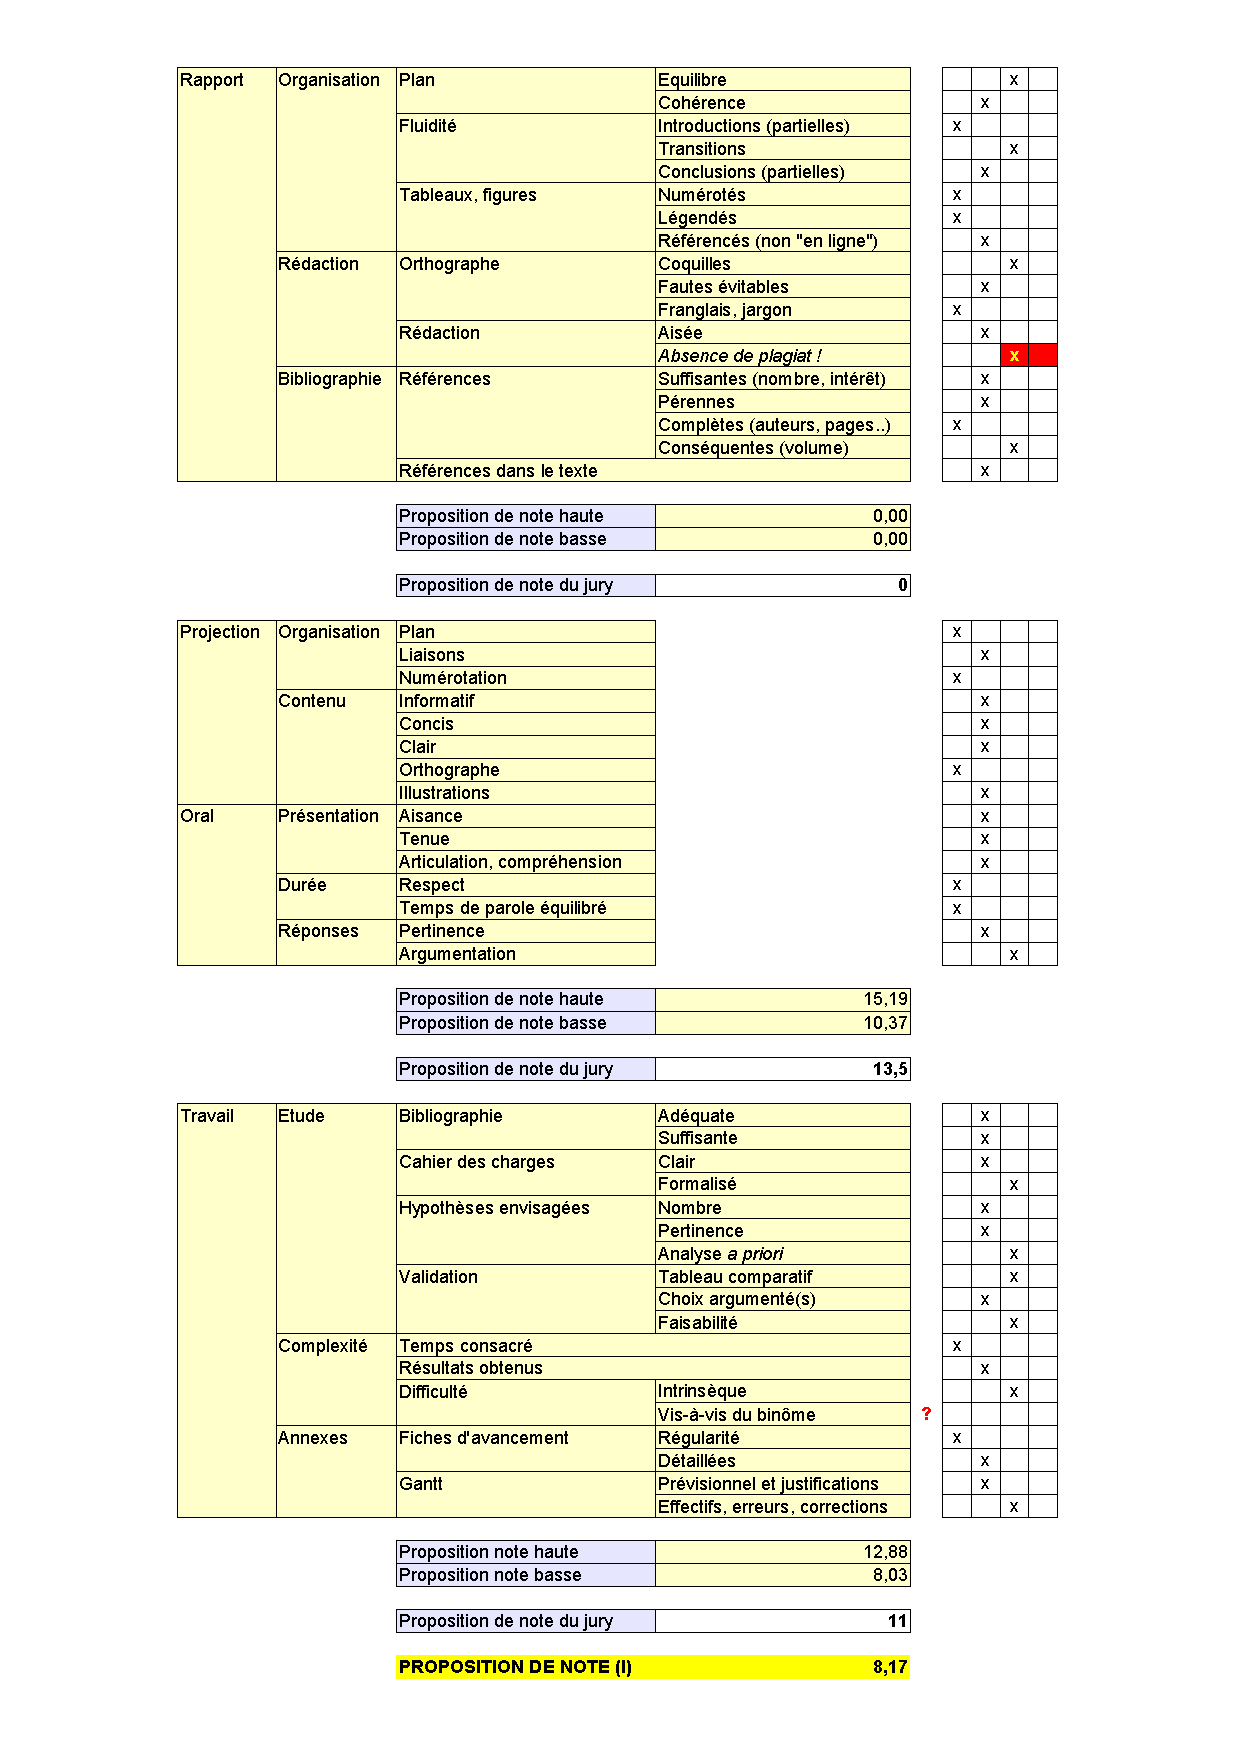
\includegraphics[width=0.9\textheight]{Images/Grille-Evaluation-PRD1}}
      \else
         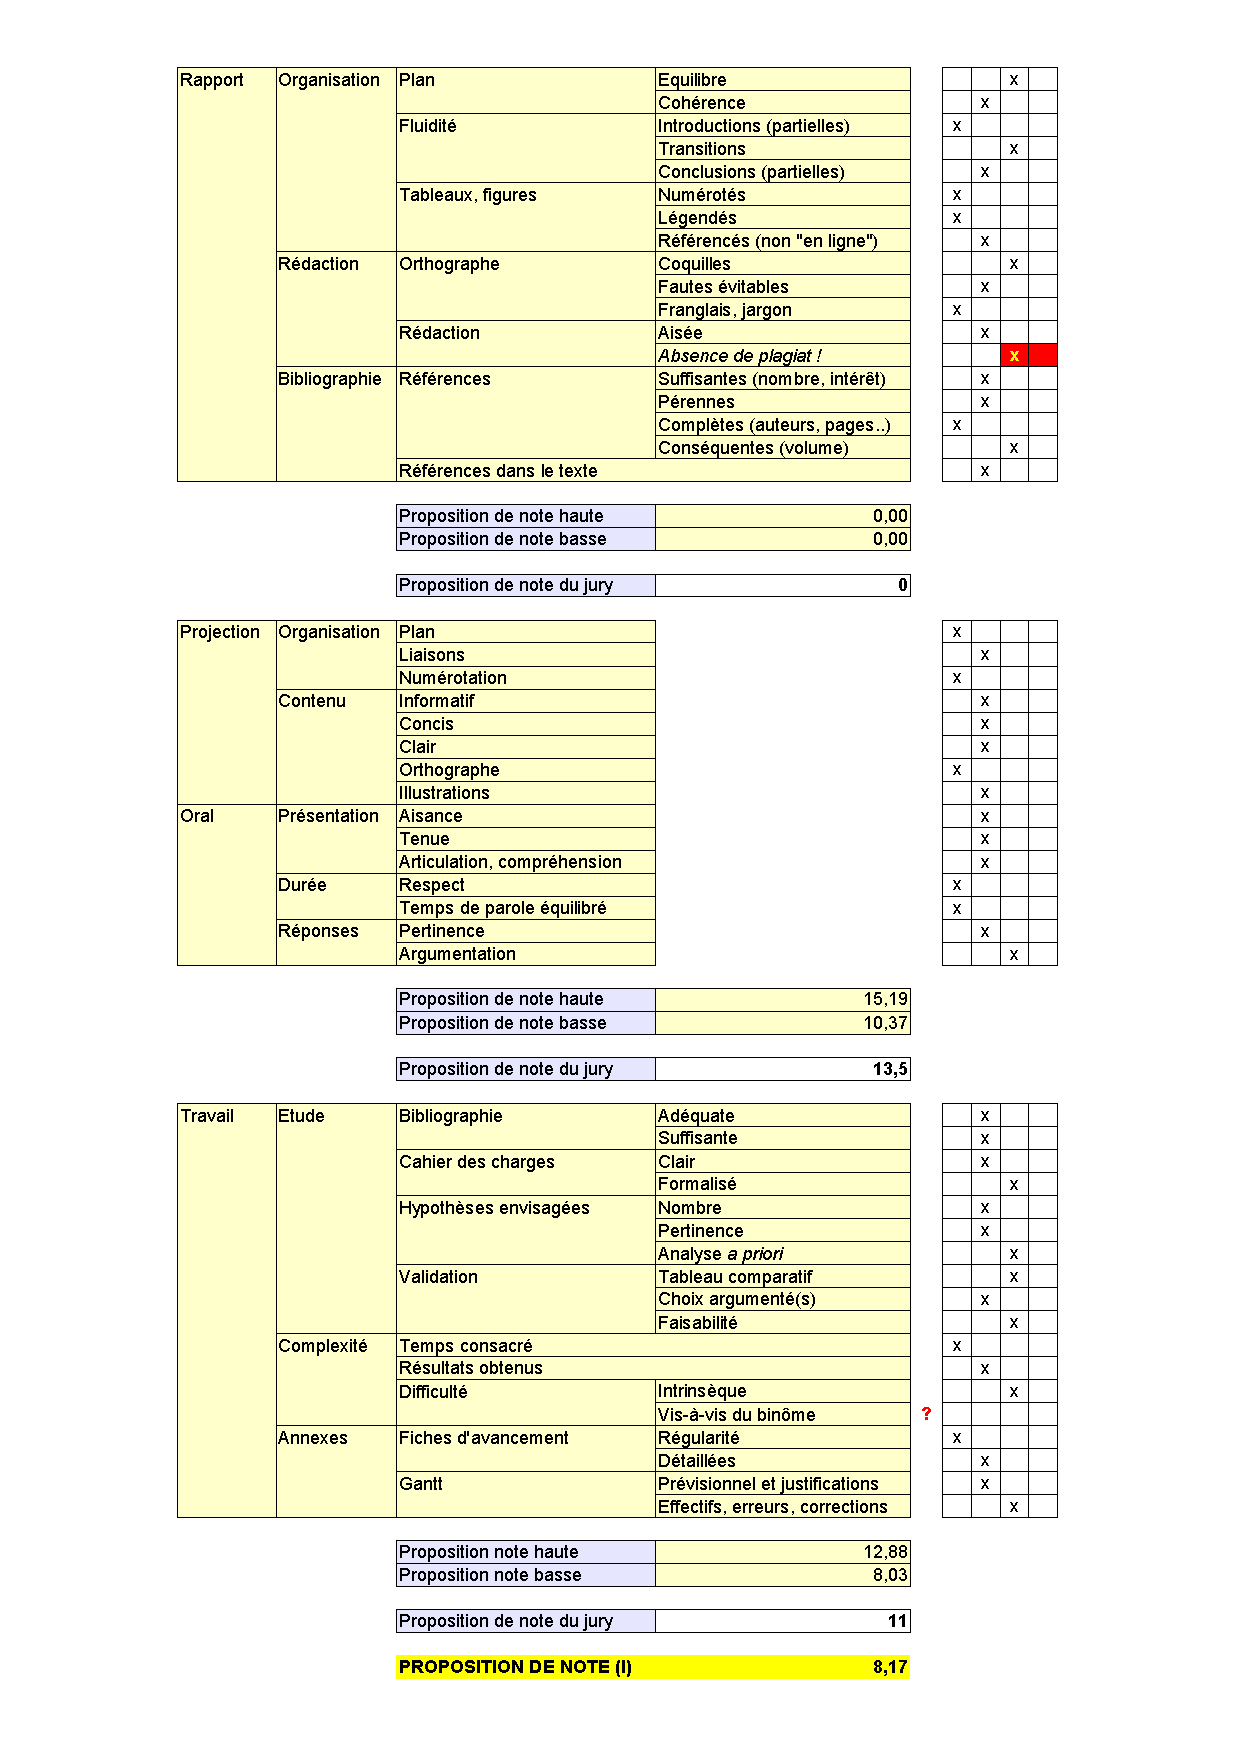
\includegraphics[width=0.9\textwidth]{Images/Grille-Evaluation-PRD1}
      \fi
   \caption{Points à contrôler à l'issue de la phase I}
   \label{fig:AutoEvaluationTravailIntermediaire}
\end{figure*}

\begin{explanation}
   La figure~\ref{fig:AutoEvaluationTravailFinal} permet d'énumérer un certain nombre de points importants dans les trois composantes du travail ainsi que d'évaluer notre niveau de satisfaction à l'issue de la phase~II, constituée de~:
   \begin{enumerate}
      \item la conception détaillée~;
      \item la réalisation~;
      \item la recette.
   \end{enumerate}
\end{explanation}

\begin{figure*}
   \centering
      \ifscreen
         \rotatebox{90}{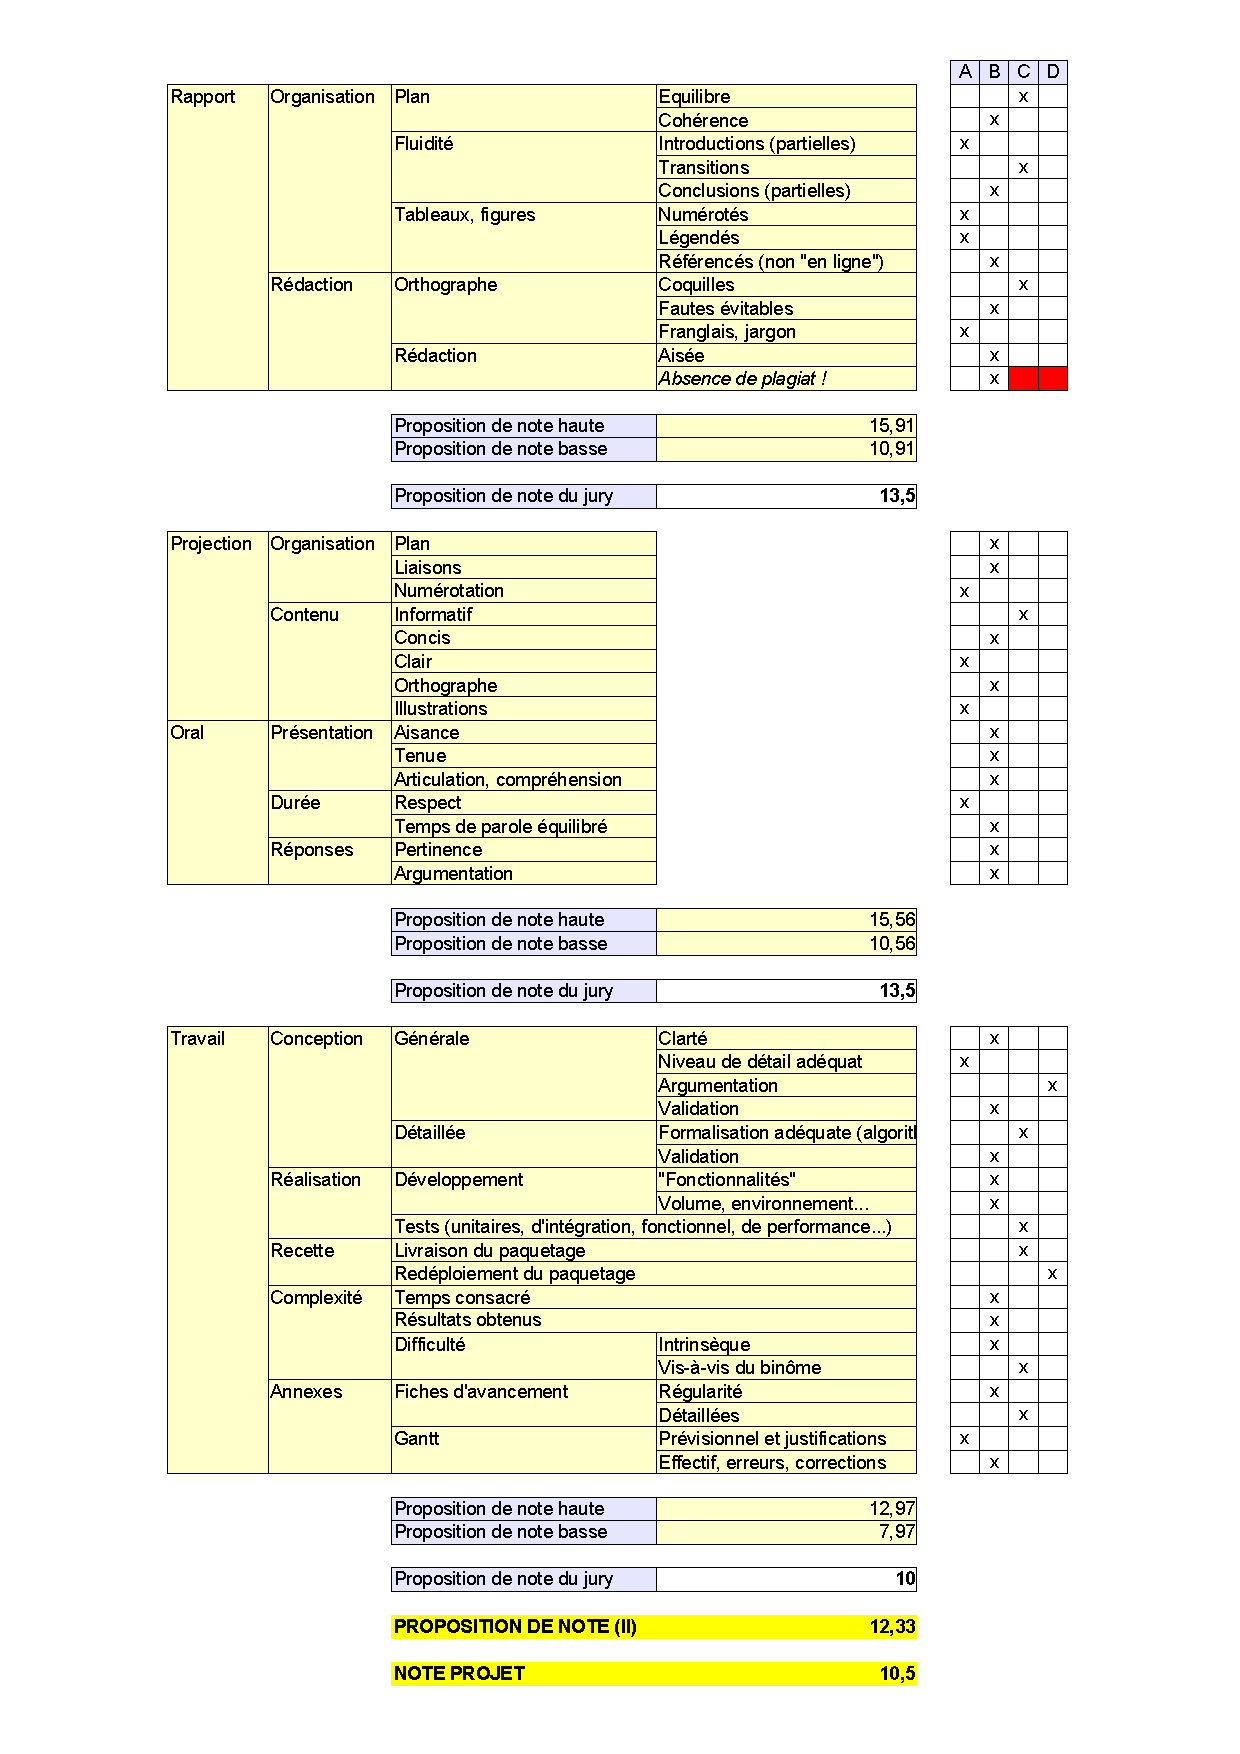
\includegraphics[width=0.9\textheight]{Images/Grille-Evaluation-PRD2}}
      \else
         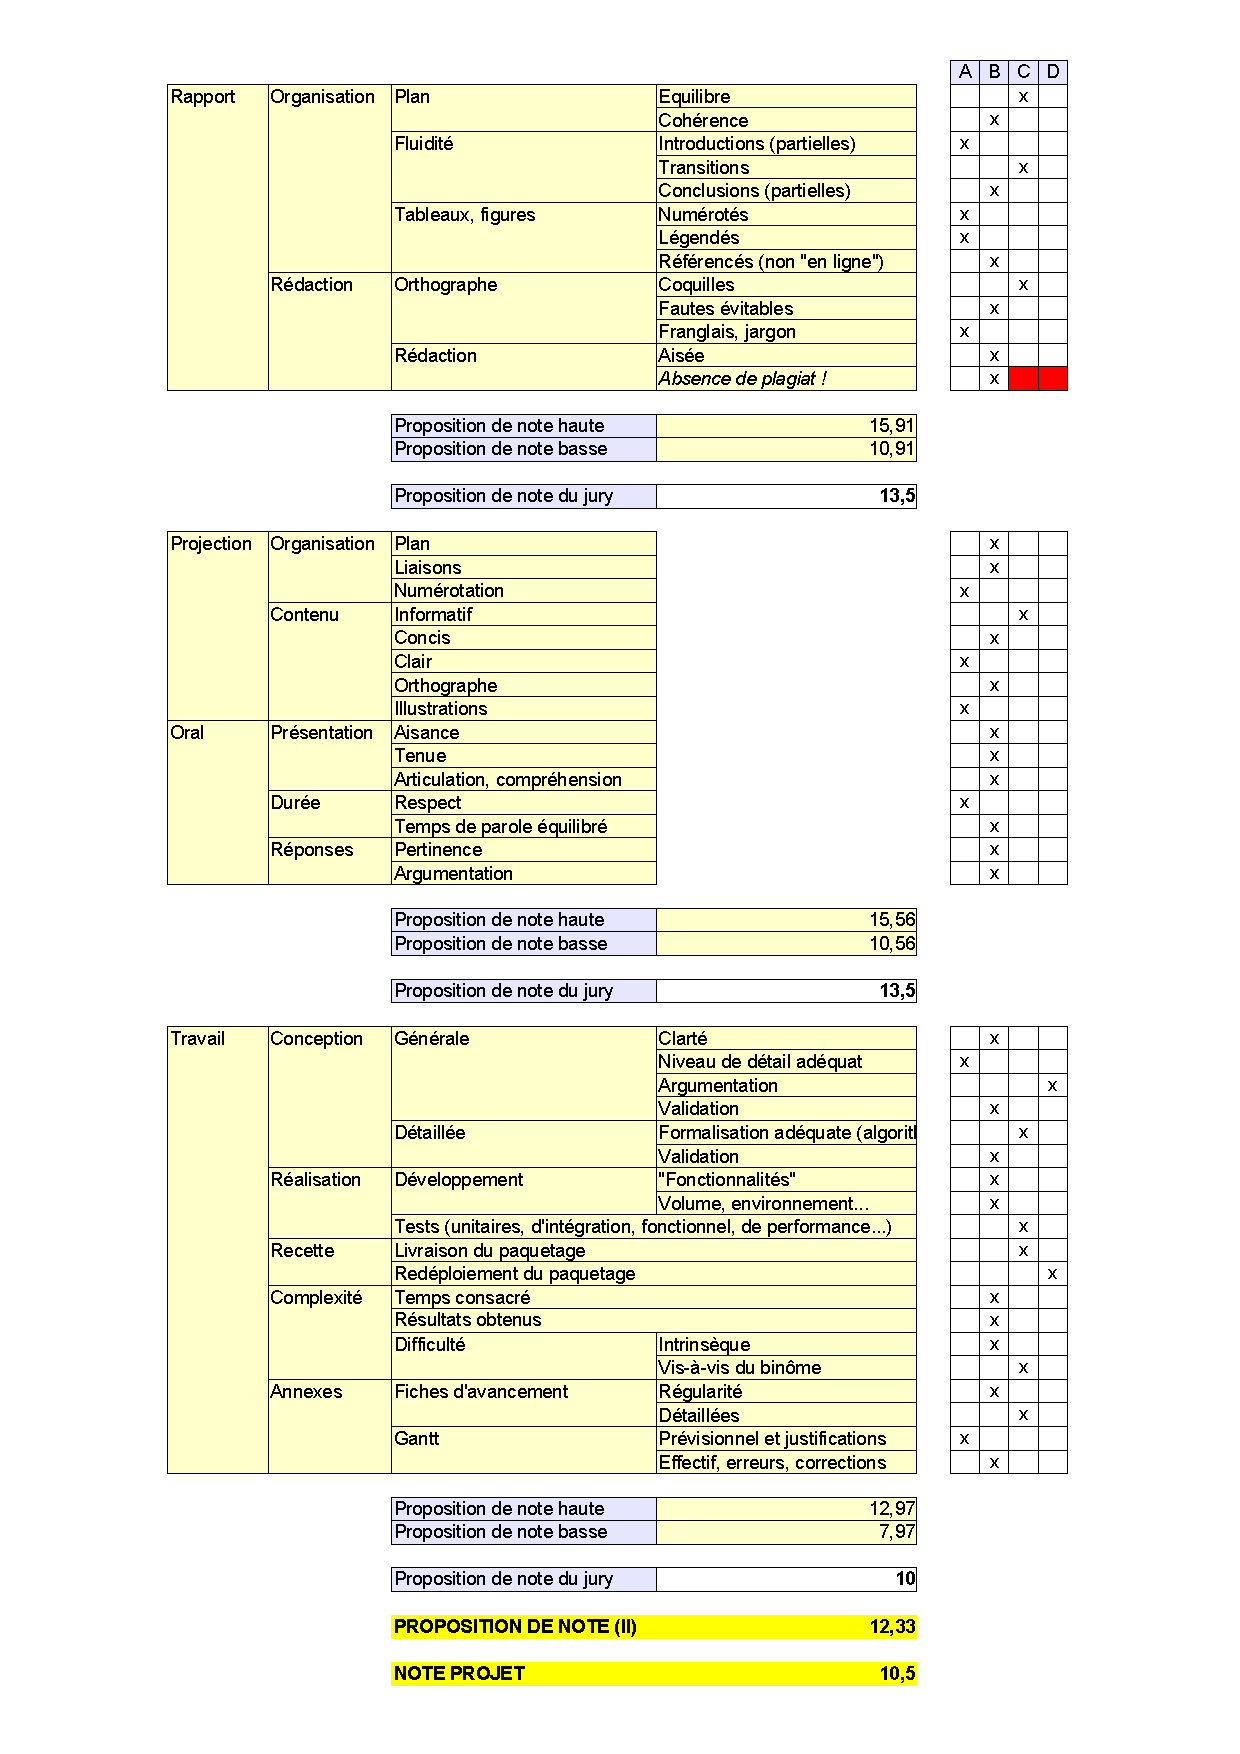
\includegraphics[width=0.9\textwidth]{Images/Grille-Evaluation-PRD2}
      \fi
   \caption{Points à contrôler à l'issue de la phase II}
   \label{fig:AutoEvaluationTravailFinal}
\end{figure*}

\end{document}

